% Options for packages loaded elsewhere
\PassOptionsToPackage{unicode}{hyperref}
\PassOptionsToPackage{hyphens}{url}
%
\documentclass[
  a4paper,
]{article}
\usepackage{lmodern}
\usepackage{amssymb,amsmath}
\usepackage{ifxetex,ifluatex}
\ifnum 0\ifxetex 1\fi\ifluatex 1\fi=0 % if pdftex
  \usepackage[T1]{fontenc}
  \usepackage[utf8]{inputenc}
  \usepackage{textcomp} % provide euro and other symbols
\else % if luatex or xetex
  \usepackage{unicode-math}
  \defaultfontfeatures{Scale=MatchLowercase}
  \defaultfontfeatures[\rmfamily]{Ligatures=TeX,Scale=1}
\fi
% Use upquote if available, for straight quotes in verbatim environments
\IfFileExists{upquote.sty}{\usepackage{upquote}}{}
\IfFileExists{microtype.sty}{% use microtype if available
  \usepackage[]{microtype}
  \UseMicrotypeSet[protrusion]{basicmath} % disable protrusion for tt fonts
}{}
\makeatletter
\@ifundefined{KOMAClassName}{% if non-KOMA class
  \IfFileExists{parskip.sty}{%
    \usepackage{parskip}
  }{% else
    \setlength{\parindent}{0pt}
    \setlength{\parskip}{6pt plus 2pt minus 1pt}}
}{% if KOMA class
  \KOMAoptions{parskip=half}}
\makeatother
\usepackage{xcolor}
\IfFileExists{xurl.sty}{\usepackage{xurl}}{} % add URL line breaks if available
\IfFileExists{bookmark.sty}{\usepackage{bookmark}}{\usepackage{hyperref}}
\hypersetup{
  pdftitle={MATH2750 Introduction to Markov Processes},
  pdfauthor={Matthew Aldridge},
  hidelinks,
  pdfcreator={LaTeX via pandoc}}
\urlstyle{same} % disable monospaced font for URLs
\usepackage[margin=1in]{geometry}
\usepackage{longtable,booktabs}
% Correct order of tables after \paragraph or \subparagraph
\usepackage{etoolbox}
\makeatletter
\patchcmd\longtable{\par}{\if@noskipsec\mbox{}\fi\par}{}{}
\makeatother
% Allow footnotes in longtable head/foot
\IfFileExists{footnotehyper.sty}{\usepackage{footnotehyper}}{\usepackage{footnote}}
\makesavenoteenv{longtable}
\usepackage{graphicx,grffile}
\makeatletter
\def\maxwidth{\ifdim\Gin@nat@width>\linewidth\linewidth\else\Gin@nat@width\fi}
\def\maxheight{\ifdim\Gin@nat@height>\textheight\textheight\else\Gin@nat@height\fi}
\makeatother
% Scale images if necessary, so that they will not overflow the page
% margins by default, and it is still possible to overwrite the defaults
% using explicit options in \includegraphics[width, height, ...]{}
\setkeys{Gin}{width=\maxwidth,height=\maxheight,keepaspectratio}
% Set default figure placement to htbp
\makeatletter
\def\fps@figure{htbp}
\makeatother
\setlength{\emergencystretch}{3em} % prevent overfull lines
\providecommand{\tightlist}{%
  \setlength{\itemsep}{0pt}\setlength{\parskip}{0pt}}
\setcounter{secnumdepth}{5}
\usepackage{booktabs}

\usepackage{titlesec, environ}
\newif\ifcomm\commtrue
\NewEnviron{myanswers}{\ifcomm\BODY\fi}

\newcommand{\sectionbreak}{\clearpage}
\usepackage[]{natbib}
\bibliographystyle{plainnat}

\title{MATH2750 Introduction to Markov Processes}
\author{\href{mailto:m.aldridge@leeds.ac.uk}{Matthew Aldridge}}
\date{University of Leeds, 2020--2021}

\usepackage{amsthm}
\newtheorem{theorem}{Theorem}[section]
\newtheorem{lemma}{Lemma}[section]
\newtheorem{corollary}{Corollary}[section]
\newtheorem{proposition}{Proposition}[section]
\newtheorem{conjecture}{Conjecture}[section]
\theoremstyle{definition}
\newtheorem{definition}{Definition}[section]
\theoremstyle{definition}
\newtheorem{example}{Example}[section]
\theoremstyle{definition}
\newtheorem{exercise}{Exercise}[section]
\theoremstyle{remark}
\newtheorem*{remark}{Remark}
\newtheorem*{solution}{Solution}
\begin{document}
\maketitle

{
\setcounter{tocdepth}{2}
\tableofcontents
}
\hypertarget{home}{%
\section*{Schedule}\label{home}}
\addcontentsline{toc}{section}{Schedule}

\textbf{Week 4} (15--19 February):

\begin{itemize}
\tightlist
\item
  \protect\hyperlink{S07-classes}{\textbf{Section 7}: Class Structure}
\item
  \protect\hyperlink{S08-hitting-times}{\textbf{Section 8}: Hitting times}
\item
  \protect\hyperlink{P04}{\textbf{Problem Sheet 4}}
\item
  \protect\hyperlink{computing}{\textbf{Computational Worksheet 1}}, with \textbf{computational drop-in sessions}: Monday, Tuesday, or Wednesday (Teams)
\item
  \textbf{Lecture}: Tuesday at 1400 (Zoom)
\item
  \textbf{Workshops} on Problem Sheet 3: Monday or Tuesday (Zoom)
\item
  Non-computational \textbf{drop-in sessions}: Tuesday or Wednesday (Teams)
\end{itemize}

\textbf{Week 3} (8--12 February):

\begin{itemize}
\tightlist
\item
  \protect\hyperlink{S05-markov-chains}{\textbf{Section 5}: Discrete time Markov chains}
\item
  \protect\hyperlink{S06-examples}{\textbf{Section 6}: Examples from actuarial science}
\item
  \protect\hyperlink{P03}{\textbf{Problem Sheet 3}}
\item
  \protect\hyperlink{A1}{\textbf{Assessment 1}} due Thursday 11 February (this week) at 1400
\item
  \protect\hyperlink{computing}{\textbf{Computational Worksheet 1}}: computational drop-in sessions next week
\end{itemize}

\textbf{Week 2} (1--5 February):

\begin{itemize}
\tightlist
\item
  \protect\hyperlink{S03-gamblers-ruin}{\textbf{Section 3}: Gambler's ruin}
\item
  \protect\hyperlink{S04-ldes}{\textbf{Section 4}: Linear difference equations}
\item
  \protect\hyperlink{P02}{\textbf{Problem Sheet 2}}
\item
  \protect\hyperlink{A1}{\textbf{Assessment 1}} due Thursday 11 February (next week) at 1400
\end{itemize}

\textbf{Week 1} (25--29 January):

\begin{itemize}
\tightlist
\item
  \protect\hyperlink{S00-about}{About the module}
\item
  \protect\hyperlink{S01-stochastic-processes}{\textbf{Section 1}: Stochastic processes and the Markov property}
\item
  \protect\hyperlink{S02-random-walk}{\textbf{Section 2}: Random walks}
\item
  \protect\hyperlink{P01}{\textbf{Problem Sheet 1}}
\end{itemize}

\hypertarget{S00-about}{%
\section*{About MATH2750}\label{S00-about}}
\addcontentsline{toc}{section}{About MATH2750}

This module is \textbf{MATH2750 Introduction to Markov Processes}. The module manager and lecturer is Dr Matthew Aldridge, and my email address is \href{mailto:m.aldridge@leeds.ac.uk}{\nolinkurl{m.aldridge@leeds.ac.uk}}.

\hypertarget{about-module}{%
\subsection*{Organisation of MATH2750}\label{about-module}}
\addcontentsline{toc}{subsection}{Organisation of MATH2750}

This module lasts for 11 weeks. The first nine weeks run from 25 January to 26 March, then we break for Easter, and then the final two weeks run from 26 April to 7 May.

\hypertarget{notes}{%
\subsubsection*{Notes and videos}\label{notes}}
\addcontentsline{toc}{subsubsection}{Notes and videos}

The main way I expect you to learn the material for this course is by reading these notes and by watching the accompanying videos. I will set two sections of notes each week, for a total of 22 sections.

Reading mathematics is a slow process. Each section roughly corresponds to one lecture last year, which would have been 50 minutes. If you find yourself regularly getting through sections in much less than an hour, you're probably not reading carefully enough through each sentence of explanation and each line of mathematics, including understanding the motivation as well as checking the accuracy.

It is possible (but not recommended) to learn the material by only reading the notes and not watching the videos. It is not possible to learn the material by only watching the videos and not reading the notes.

You are probably reading the web version of the notes. If you want a PDF copy (to read offline or to print out), then click the PDF button in the top ribbon of the page. (Warning: I have not made as much effort to make the PDF neat and tidy as I have the web version.)

Since we will all be relying heavily on these notes, I'm even more keen than usual to hear about errors mathematical, typographical or otherwise. Please, please \href{mailto:m.aldridge@leeds.ac.uk}{email me} if think you may have found any.

\hypertarget{problem-sheets}{%
\subsubsection*{Problem sheets}\label{problem-sheets}}
\addcontentsline{toc}{subsubsection}{Problem sheets}

There will be 10 problem sheets; Problem Sheet \(n\) covers the material from the two sections from week \(n\) (Sections \(2n -1\) and \(2n\)), and will be discussed in your workshop in week \(n+1\).

\hypertarget{lectures}{%
\subsubsection*{Lectures}\label{lectures}}
\addcontentsline{toc}{subsubsection}{Lectures}

There will be one online synchronous ``lecture'' session each week, on Tuesdays at 1400, with me, run through Zoom.

This will not be a ``lecture'' in the traditional sense of the term, but will be an opportunity to re-emphasise material you have already learned from notes and videos, to give extra examples, and to answer common student questions, with some degree of interactivity.

I will assume you have completed all the work for the previous week by the time of the lecture, but I will not assume you've started the work for that week itself.

I am very keen to hear about things you'd like to go through in the lectures; please \href{mailto:m.aldridge@leeds.ac.uk}{email me} with your suggestions.

\hypertarget{workshops}{%
\subsubsection*{Workshops}\label{workshops}}
\addcontentsline{toc}{subsubsection}{Workshops}

There will be 10 workshops, starting in the second week. The main goal of the workshops will be to go over your answers to the problems sheets in smaller classes. You will have been assigned to one of three workshop groups, meeting on Mondays or Tuesdays, led by \href{https://eps.leeds.ac.uk/maths/pgr/8790/jason-klebes}{Jason Klebes}, \href{http://www1.maths.leeds.ac.uk/~voss/}{Dr Jochen Voss}, or me. Your workshop will be run through Zoom or Microsoft Teams; your workshop leader will contact you before the end of this week with arrangements.

My recommended approach to problem sheets and workshops is the following:

\begin{itemize}
\tightlist
\item
  Work through the problem sheet before the workshop, spending plenty of time on it, and making multiple efforts at questions you get stuck on. I recommend spending \emph{at least three hours} on each problem sheet, in more than one block. Collaboration is encouraged when working through the problems, but I recommend writing up your work on your own.
\item
  Take advantage of the smaller group setting of the workshop to ask for help or clarification on questions you weren't able to complete.
\item
  After the workshop, attempt again the questions you were previously stuck on.
\item
  If you're still unable to complete a question after this second round of attempts, \emph{then} consult the solutions.
\end{itemize}

\hypertarget{assessments}{%
\subsubsection*{Assessments}\label{assessments}}
\addcontentsline{toc}{subsubsection}{Assessments}

There will be four pieces of assessed coursework, making up a total of 15\% of your mark for the module. Assessments 1, 3 and 4 will involve writing up answers to a few problems, in a similar style to the problem sheets, and are worth 4\% each. (In response to previous student feedback, there are fewer questions per assessment.) Assessment 2 will be a report on some computational work (\protect\hyperlink{about--computing}{see below}) and is worth 3\%.

Copying, plagiarism and other types of cheating are not allowed and will be dealt with in accordance with University procedures.

The assessments deadlines are:

\begin{itemize}
\tightlist
\item
  Assessment 1: Thursday 11 February 1400 (week 3)
\item
  Assessment 2 (Computational Worksheet 2): Thursday 18 March 1400 (week 8)
\item
  Assessment 3: Thursday 25 March 1400 (week 9)
\item
  Assessment 4: Thursday 6 May 1400 (week 11)
\end{itemize}

Work will be submitted via Gradescope.

Your markers are Jason Klebes, Macauley Locke, and Muyang Zhang -- but you should \href{mailto:m.aldridge@leeds.ac.uk}{contact the module leader} if you have marking queries, not the markers directly.

\hypertarget{about-computing}{%
\subsubsection*{Computing worksheets}\label{about-computing}}
\addcontentsline{toc}{subsubsection}{Computing worksheets}

There will be two computing worksheets, which will look at the material in the course through simulations in R. This material is examinable. You should be able to work through the worksheets in your own time, but if you need help, there will be optional online drop-in sessions in the weeks 4 and 7 with \href{https://eps.leeds.ac.uk/maths/pgr/6422/muyang-zhang}{Muyang Zhang} through Microsoft Teams. (Your computing drop-in session may be listed as ``Practical'' on your timetable.)

The first computing worksheet will be a practice run, while a report on the second computing worksheet will be the second assessed piece of work.

\hypertarget{dropin}{%
\subsubsection*{Drop-in sessions}\label{dropin}}
\addcontentsline{toc}{subsubsection}{Drop-in sessions}

If you there is something in the course you wish to discuss in detail, the place for the is the optional weekly drop-in session. The drop-in sessions are an optional opportunity for you to ask questions you have to a member of staff -- nothing will happen unless you being your questions.

You will have been assigned to one of three groups on Tuesdays or Wednesdays with \href{https://eps.leeds.ac.uk/maths/pgr/4992/nikita-merkulov}{Nikita Merkulov} or me. The drop-in sessions will be run the Microsoft Teams. Your drop-in session would be an excellent place to go if you are having trouble understanding something in the written notes, or if you're still struggling on a problem sheet question after your workshop.

\hypertarget{team}{%
\subsubsection*{Microsoft Team}\label{team}}
\addcontentsline{toc}{subsubsection}{Microsoft Team}

I have set up \href{https://teams.microsoft.com/l/channel/19\%3a8cb8008c95204bbeaefa8ee7d48c1a13\%40thread.tacv2/General?groupId=1c138eac-0c54-43b0-9d20-d4cf3d65c40a\&tenantId=bdeaeda8-c81d-45ce-863e-5232a535b7cb}{a Microsoft Team} for the course. I propose to use the ``Q and A'' channel there as a discussion board. This is a good place to post questions about material from the course, and -- even better! -- to help answer you colleagues' questions. The idea is that you all as a group should help each other out. I will visit a couple of times a week to clarify if everybody is stumped by a question, or if there is disagreement.

\hypertarget{time}{%
\subsubsection*{Time management}\label{time}}
\addcontentsline{toc}{subsubsection}{Time management}

It is, of course, up to you how you choose to spend your time on this module. But, if you're interested, my recommendations would be something like this:

\begin{itemize}
\tightlist
\item
  \textbf{Every week:} 7.5 hours per week

  \begin{itemize}
  \tightlist
  \item
    \textbf{Notes and videos:} 2 sections, 1 hour each
  \item
    \textbf{Problem sheet:} 3.5 hours per week
  \item
    \textbf{Lecture:} 1 hour per week
  \item
    \textbf{Workshop:} 1 hour per week
  \end{itemize}
\item
  \textbf{When required:}

  \begin{itemize}
  \tightlist
  \item
    \textbf{Assessments 1, 2 and 4:} 2 hours each
  \item
    \textbf{Computer worksheets:} 2 hours each
  \item
    \textbf{Revision}: 12 hours
  \end{itemize}
\item
  \textbf{Total:} 100 hours
\end{itemize}

\hypertarget{exam}{%
\subsubsection*{Exam}\label{exam}}
\addcontentsline{toc}{subsubsection}{Exam}

There will be an exam -- or, rather, a final ``online time-limited assessment'' -- after the end of the module, making up the remaining 85\% of your mark. The exam will consist of four questions, and you are expected to answer all of them. You will have 48 hours to complete the exam, although the exam itself should represent half a day to a day's work. Further details to follow nearer the time.

\hypertarget{ask}{%
\subsubsection*{Who should I ask about\ldots?}\label{ask}}
\addcontentsline{toc}{subsubsection}{Who should I ask about\ldots?}

\begin{itemize}
\tightlist
\item
  \emph{I don't understand something in the notes or on a problem sheet}: Go to your weekly drop-in session, or post a question on \href{https://teams.microsoft.com/l/channel/19\%3a5fcd058b7074426ca1f7d1cf2052d3b4\%40thread.tacv2/Q\%2520and\%2520A?groupId=1c138eac-0c54-43b0-9d20-d4cf3d65c40a\&tenantId=bdeaeda8-c81d-45ce-863e-5232a535b7cb}{the Teams Q and A board}. (If you email me, I am likely to respond, ``That would be an excellent question for your drop-in session or the Q and A board.'')
\item
  \emph{I don't understand something in on a computational worksheet:} Go to your computing drop-in session in weeks 4 or 7.
\item
  \emph{I have an admin question about general arrangements for the module:} \href{mailto:m.aldridge@leeds.ac.uk}{Email me}.
\item
  \emph{I have an admin question about arrangements for my workshop:} Email your workshop leader.
\item
  \emph{I have suggestion for something to cover in the lectures:} \href{mailto:m.aldridge@leeds.ac.uk}{Email me}.
\item
  \emph{I need an extension on or exemption from an assessment:} \href{mailto:Maths.Taught.Students@leeds.ac.uk}{Email the Maths Taught Students Office}.
\end{itemize}

\hypertarget{about-content}{%
\subsection*{Content of MATH2750}\label{about-content}}
\addcontentsline{toc}{subsection}{Content of MATH2750}

\hypertarget{prereqs}{%
\subsubsection*{Prerequisites}\label{prereqs}}
\addcontentsline{toc}{subsubsection}{Prerequisites}

Some students have asked what background you'll be expected to know for this course.

It's essential that you're very comfortable with the basics of probability theory: events, probability, discrete and continuous random variables, expectation, variance, approximations with the normal distribution, etc. Conditional probability and independence are particularly important concepts in this course. This course will use the binomial, geometric, Poisson, normal and exponential distributions, although the notes will usually remind you about them first, in case you've forgotten.

Many students on the module will have studied these topics in MATH1710 Probability and Statistics 1; others will have covered these in different modules.

\hypertarget{syllabus}{%
\subsubsection*{Syllabus}\label{syllabus}}
\addcontentsline{toc}{subsubsection}{Syllabus}

The course has two major parts: the first part will cover processes in discrete time and the second part processes in continuous time.

An outline plan of the topics covered is the following. (Remember that one week's work is two sections of notes.)

\begin{itemize}
\tightlist
\item
  \textbf{Discrete time Markov chains} {[}12 sections{]}

  \begin{itemize}
  \tightlist
  \item
    Introduction to stochastic processes {[}1 section{]}
  \item
    Important examples: Random walk, gambler's ruin, linear difference equations, examples from actuarial science {[}4 sections{]}
  \item
    General theory: transition probabilities, \(n\)-step transition probabilities, class structure, periodicity, hitting times, recurrence and transience, stationary distributions, long-term behaviour {[}6 sections{]}
  \item
    Revision {[}1 section{]}
  \end{itemize}
\item
  \textbf{Continuous time Markov jump processes} {[}10 sections{]}

  \begin{itemize}
  \tightlist
  \item
    Important examples: Poisson process, counting processes, queues {[}5 sections{]}
  \item
    General theory: holding times and jump chains, forward and backward equations, class structure, hitting times, stationary distributions, long-term behaviour {[}4 sections{]}
  \item
    Revision {[}1 section{]}
  \end{itemize}
\end{itemize}

\hypertarget{books}{%
\subsubsection*{Books}\label{books}}
\addcontentsline{toc}{subsubsection}{Books}

You can do well on this module by reading the notes and watching the videos, attending the lectures and workshops, and working on the problem sheets, assignments and practicals, without any further reading. However, students can benefit from optional extra background reading or an alternative view on the material.

My favourite book on Markov chains, which I used a lot while planning this course and writing these notes, is:

\begin{itemize}
\tightlist
\item
  J.R. Norris, \emph{Markov Chains}, Cambridge Series in Statistical and Probabilistic Mathematics, Cambridge University Press, 1997. Chapters 1-3.
\end{itemize}

This a whole book just on Markov processes, including some more detailed material that goes beyond this module. Its coverage of of both discrete and continuous time Markov processes is very thorough. \href{http://www.statslab.cam.ac.uk/~james/Markov/}{Chapter 1 on discrete time Markov chains is available online.}

Other good books with sections on Markov processes that I have used include:

\begin{itemize}
\tightlist
\item
  G.R. Grimmett and D.R. Stirzaker, \emph{Probability and Random Processes}, 4th edition, Oxford University Press, 2020. Chapter 6.
\item
  G. Grimmet and D. Walsh, \emph{Probability: an introduction}, 2nd edition, Oxford University Press, 2014. Chapter 12.
\item
  D.R. Stirzaker, \href{https://leeds.primo.exlibrisgroup.com/permalink/44LEE_INST/13rlbcs/alma991013131349705181}{\emph{Elementary Probability}}, 2nd edition, Cambridge University Press, 2003. Chapter 9.
\end{itemize}

Grimmett and Stirzaker is an excellent handbook that covers most of undergraduate probability -- I bought a copy when I was a second-year undergraduate and still keep it next to my desk.
\href{https://leeds.primo.exlibrisgroup.com/permalink/44LEE_INST/13rlbcs/alma991013131349705181}{The whole of Stirzaker is available online.}

A gentler introduction with plenty of examples is provided by:

\begin{itemize}
\tightlist
\item
  P.W. Jones and P. Smith, \href{https://leeds.primo.exlibrisgroup.com/permalink/44LEE_INST/13rlbcs/alma991002938739705181}{\emph{Stochastic Processes: an introduction}}, 3nd edition, Texts in Statistical Science, CRC Press, 2018. Chapters 2-7.
\end{itemize}

although it doesn't cover everything in this module. \href{https://leeds.primo.exlibrisgroup.com/permalink/44LEE_INST/13rlbcs/alma991002938739705181}{The whole book is available online.}

(I've listed the newest editions of these books, but older editions will usually be fine too.)

\hypertarget{finally}{%
\subsubsection*{And finally\ldots{}}\label{finally}}
\addcontentsline{toc}{subsubsection}{And finally\ldots{}}

These notes were mostly written by Matthew Aldridge in 2018--19, and have received updates (mostly in Sections 9--11) and reformatting this year. Some of the material (especially Section 1, Section 6, and numerous diagrams) follows closely previous notes by Dr Graham Murphy, and I also benefited from reading earlier notes by Dr Robert Aykroyd and Prof Alexander Veretennikov. Dr Murphy's general help and advice was also very valuable. Many thanks to students in previous runnings of the module for spotting errors and suggesting improvements.

\hypertarget{part-part-i-discrete-time-markov-chains}{%
\part*{Part I: Discrete time Markov chains}\label{part-part-i-discrete-time-markov-chains}}
\addcontentsline{toc}{part}{Part I: Discrete time Markov chains}

\hypertarget{S01-stochastic-processes}{%
\section{Stochastic processes and the Markov property}\label{S01-stochastic-processes}}

\begin{itemize}
\tightlist
\item
  Stochastic processes with discrete or continuous state space and discrete or continuous time
\item
  The Markov ``memoryless'' property
\end{itemize}

\hypertarget{models}{%
\subsection{Deterministic and random models}\label{models}}

A \textbf{model} is an imitation of a real-world system. For example, you might want to have a model to imitate the world's population, the level of water in a reservoir, cashflows of a pension scheme, or the price of a stock. Models allow us to try to understand and predict what might happen in the real world in a low risk, cost effective and fast way.

To design a model requires a set of assumptions about how it will work and suitable parameters need to be determined, perhaps based on past collected data.

An important distinction is between \textbf{deterministic} models and \textbf{random} models. Another word for a random model is a \textbf{stochastic} (``\emph{sto}-\textsc{\emph{kass}}-\emph{tik}'') model. Deterministic models do not contain any random components, so the output is completely determined by the inputs and any parameters. Random models have variable outcomes to account for uncertainty and unpredictability, so they can be run many times to give a sense of the range of possible outcomes.

Consider models for:

\begin{itemize}
\tightlist
\item
  the future position of the Moon as it orbits the Earth,
\item
  the future price of shares in Apple.
\end{itemize}

For the moon, the random components -- for example, the effect of small meteorites striking the Moon's surface -- are not very significant and a deterministic model based on physical laws is good enough for most purposes. For Apple shares, the price changes from day to day are highly uncertain, so a random model can account for the variability and unpredictability in a useful way.

In this module we will see many examples of stochastic models. Lots of the applications we will consider come from financial mathematics and actuarial science where the use of models that take into account uncertainty is very important, but the principles apply in many areas.

\hypertarget{stochastic-processes}{%
\subsection{Stochastic processes}\label{stochastic-processes}}

If we want to model, for example, the total number of claims to an insurance company in the whole of 2020, we can use a random variable \(X\) to model this -- perhaps a Poisson distribution with an appropriate mean. However, if we want to track how the number of claims changes over the course of the year 2021, we will need to use a \textbf{stochastic process} (or ``random process'').

A stochastic process, which we will usually write as \((X_n)\), is an indexed sequence of random variables that are (usually) dependent on each other.

Each random variable \(X_n\) takes a value in a \textbf{state space} \(\mathcal S\) which is the set of possible values for the process. As with usual random variables, the state space \(\mathcal S\) can be \textbf{discrete} or \textbf{continuous}. A discrete state space denotes a set of distinct possible outcomes, which can be finite or countably infinite. For example, \(\mathcal S = \{\text{Heads},\text{Tails}\}\) is the state space for a single coin flip, while in the case of counting insurance claims, the state space would be the nonnegative integers \(\mathcal S = \mathbb Z_+ = \{0,1,2,\dots\}\). A continuous state space denotes an uncountably infinite continuum of gradually varying outcomes. For example, the nonnegative real line \(\mathcal S = \mathbb R_+ = \{x \in \mathbb R : x \geq 0\}\) is the state space for the amount of rainfall on a given day, while some bounded subset of \(\mathbb R^3\) would be the state space for the position of a gas particle in a box.

Further, the process has an \textbf{index set} that puts the random variables that make up the process in order. The index set is usually interpreted as a \textbf{time} variable, telling us when the process will be measured. The index set for time can also be discrete or continuous. Discrete time denotes a process sampled at distinct points, often denoted by \(n = 0,1,2,\dots\), while continuous time denotes a process monitored constantly over time, often denoted by \(t \in \mathbb R_+ = \{x \in \mathbb R : x \geq 0\}\). In the insurance example, we might count up the number of claims each day -- then the discrete index set will be the days of the year, which we could denote \(\{1,2,\dots,365\}\). Alternatively, we might want to keep a constant tally that we update after every claim, requiring a continuous time index \(t\) representing time across the whole year. In discrete time, we can write down the first few steps of the process as \((X_0, X_1, X_2, \dots)\).

This gives us four possibilities in total:

\begin{itemize}
\tightlist
\item
  \textbf{Discrete time, discrete space}

  \begin{itemize}
  \tightlist
  \item
    Example: Number of students attending each lecture of maths module.
  \item
    \textbf{Markov chains} -- discrete time, discrete space stochastic processes with a certain ``Markov property'' -- are the main topic of the first half of this module.
  \end{itemize}
\item
  \textbf{Discrete time, continuous space}

  \begin{itemize}
  \tightlist
  \item
    Example: Daily maximum temperature in Leeds.
  \item
    We will briefly mention continuous space Markov chains in the first half of the course, but these are not as important.
  \end{itemize}
\item
  \textbf{Continuous time, discrete space}

  \begin{itemize}
  \tightlist
  \item
    Example: Number of visitors to a webpage over time.
  \item
    \textbf{Markov jump processes} -- continuous time, discrete space stochastic processes with the ``Markov property'' -- are the main topic of the second half of this module.
  \end{itemize}
\item
  \textbf{Continuous time, continuous space}

  \begin{itemize}
  \tightlist
  \item
    Example: Level of the FTSE 100 share index over time.
  \item
    Such processes, especially the famous Brownian motion -- another process with the Markov property -- are very important, but outside the scope of this course. See MATH3734 Stochastic Calculus for Finance next year, for example.
  \end{itemize}
\end{itemize}

\hypertarget{markov-property}{%
\subsection{Markov property}\label{markov-property}}

Because stochastic processes consist of a large number -- even infinitely many; even uncountably infinitely many -- random variables that could all be dependent on each other, they can get extremely complicated. The Markov property is a crucial property that restricts the type of dependencies in a process, to make the process easier to study, yet still leaves most of the useful and interesting examples intact. (Although particular examples of Markov processes go back further, the first general study was by the Russian mathematician \href{https://mathshistory.st-andrews.ac.uk/Biographies/Markov/}{Andrey Andreyevich Markov}, published in 1906.)

Think of a simple board game where we roll a dice and move that many squares forward on the board. Suppose we are currently on the square \(X_n\). Then what can we say about which square \(X_{n+1}\) we move to on our next turn?

\begin{itemize}
\tightlist
\item
  \(X_{n+1}\) is random, since it depends on the roll of the dice.
\item
  \(X_{n+1}\) depends on where we are now \(X_n\), since the score of dice will be added onto the number our current square,
\item
  Given the square \(X_n\) we are now, \(X_{n+1}\) doesn't depend any further on which sequence of squares \(X_0, X_1, \dots, X_{n-1}\) we used to get here.
\end{itemize}

It is this third point that is the crucial property of the stochastic processes we will study in this course, and it is called the \textbf{Markov property} or \textbf{memoryless property}. We say ``memoryless'', because it's as if the process forgot how it got here -- we only need to remember what square we've reached, not which squares we used to get here. The stochastic process before this moment has no bearing on the future, given where we are now. A mathematical way to say this is that ``the past and the future are conditionally independent given the present.''

To write this down formally, we need to recall \textbf{conditional probability}: the conditional probability of an event \(A\) given another event \(B\) is written \(\mathbb P(A \mid B)\), and is the probability that \(A\) occurs \emph{given} that \(B\) definitely occurs. You may remember the definition
\[ \mathbb P(A \mid B) = \frac{\mathbb P(A \cap B)}{\mathbb P(B)} , \]
although is often more useful to reason directly about conditional probabilities than use this formula.

(You may also remember that the definition of conditional probability requires that \(\mathbb P(B) > 0\). Whenever we write down a conditional probability, we implicitly assume the conditioning event has strictly positive probability without explicitly saying so.)

\begin{definition}
\protect\hypertarget{def:def-markov-property}{}\label{def:def-markov-property}

Let \((X_n) = (X_0, X_1, X_2, \dots)\) be a stochastic process in discrete time \(n = 0,1,2,\dots\) and discrete space \(\mathcal S\). Then we say that \((X_n)\) has the \textbf{Markov property} if, for all times \(n\) and all states \(x_0, x_1, \dots,x_n, x_{n+1} \in \mathcal S\) we have
\[  \mathbb P(X_{n+1}=x_{n+1} \mid X_{n}=x_{n}, X_{n-1} = x_{n-1}, \dots,X_0=x_0) = \mathbb P(X_{n+1}=x_{n+1} \mid X_{n}=x_{n}) . \]

\end{definition}

Here, the left hand side is the probability we go to state \(x_{n+1}\) next conditioned on the entire history of the process, while the right hand side is the probability we go to state \(x_{n+1}\) next conditioned only on where we are now \(x_n\). So the Markov property tells us that it only matters where we are now and not how we got here.

(There's also a similar definition for continuous time processes, which we'll come to later in the course.)

Stochastic processes that have the Markov property are much easier to study than general processes, as we only have to keep track of where we are now and we can forget about the entire history that came before.

\textbf{In the next section}, we'll see the first, and most important, example of a discrete time discrete space Markov chain: the ``random walk''.

\hypertarget{S02-random-walk}{%
\section{Random walk}\label{S02-random-walk}}

\newcommand{\Var}{\operatorname{Var}}

\begin{itemize}
\tightlist
\item
  Definition of the simple random walk and the exact binomial distribution
\item
  Expectation and variance of general random walks
\end{itemize}

\hypertarget{simple-random-walk}{%
\subsection{Simple random walk}\label{simple-random-walk}}

Consider the following \textbf{simple random walk} on the integers \(\mathbb Z\): We start at \(0\), then at each time step, we go up by one with probability \(p\) and down by one with probability \(q = 1-p\). When \(p = q = \frac12\), we're equally as likely to go up as down, and we call this the \textbf{simple symmetric random walk}.

The simple random walk is a simple but very useful model for lots of processes, like stock prices, sizes of populations, or positions of gas particles. (In many modern models, however, these have been replaced by more complicated continuous time and space models.) The simple random walk is sometimes called the ``drunkard's walk'', suggesting it could model a drunk person trying to stagger home.

\begin{figure}
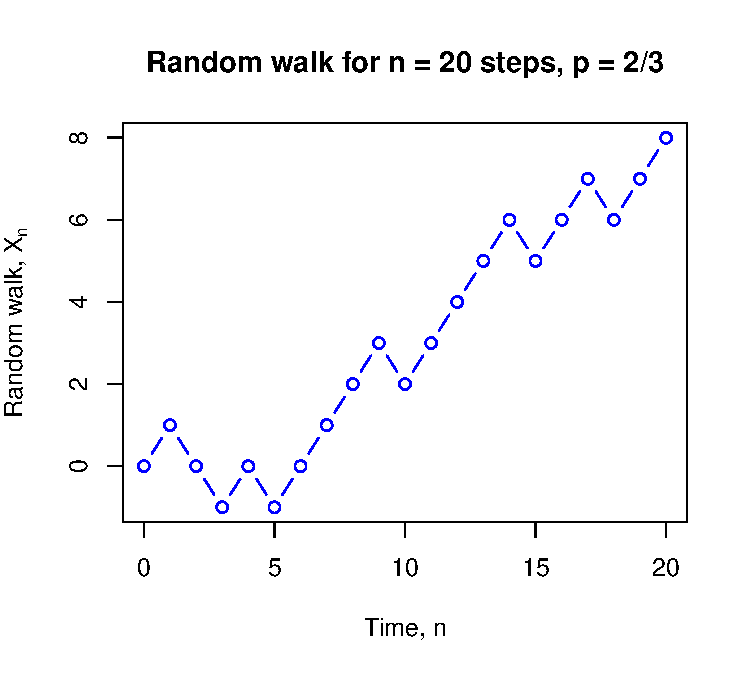
\includegraphics[width=0.5\linewidth]{math2750_files/figure-latex/rw-pics-1} 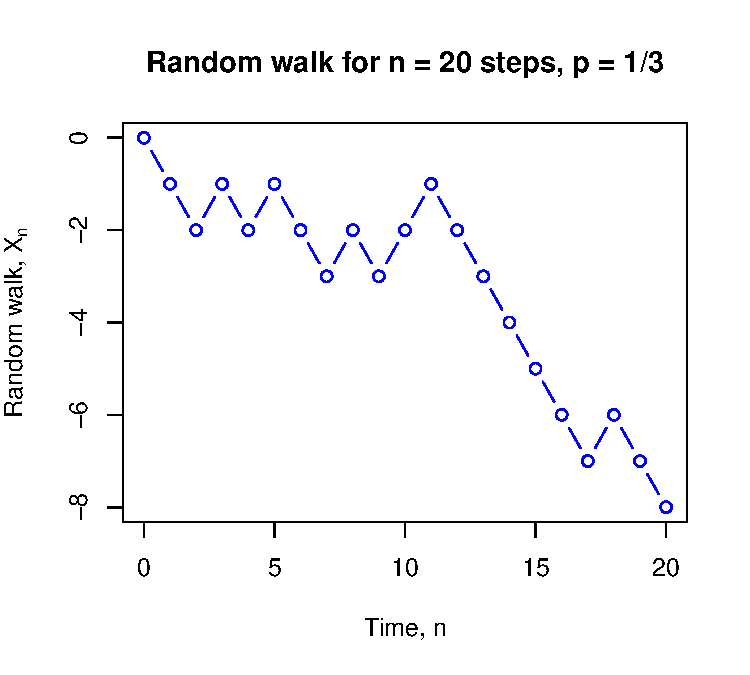
\includegraphics[width=0.5\linewidth]{math2750_files/figure-latex/rw-pics-2} \caption{Two simulations of random walks.}\label{fig:rw-pics}
\end{figure}

We can write this as a stochastic process \((X_n)\) with discrete time \(n = \{0,1,2,\dots\} = \mathbb Z_+\) and discrete state space \(\mathcal S = \mathbb Z\), where \(X_0 = 0\) and, for \(n \geq 0\), we have
\[ X_{n+1} = \begin{cases} X_n + 1 & \text{with probability $p$,} \\
                             X_n - 1 & \text{with probability $q$.} \end{cases} \]

It's clear from this definition that \(X_{n+1}\) (the future) depends on \(X_n\) (the present), but, given \(X_n\), does not depend on \(X_{n-1}, \dots, X_1, X_0\) (the past). Thus the Markov property holds, and the simple random walk is a \textbf{discrete time Markov process} or \textbf{Markov chain}.

\begin{example}
\protect\hypertarget{exm:rw1}{}\label{exm:rw1}

\emph{What is the probability that after two steps a simple random walk has reached \(X_2 = 2\)?}

To achieve this, the walk must go upwards in both time steps, so \(\mathbb P(X_2 = 2) = pp = p^2\).

\end{example}

\begin{example}
\protect\hypertarget{exm:rw2}{}\label{exm:rw2}

\emph{What is the probability that after three steps a simple random walk has reached \(X_3 = -1\)?}

There are three ways to reach \(-1\) after three steps: up--down--down, down--up--down, or down--down--up. So
\[ \mathbb P(X_3 = -1) = pqq+qpq+qqp = 3pq^2 . \]

\end{example}

\hypertarget{general-random-walks}{%
\subsection{General random walks}\label{general-random-walks}}

An alternative way to write the simple random walk is to put
\begin{equation}
    X_n = X_0 + \sum_{i=1}^n Z_i ,  \label{eq:rw}
  \end{equation}
where the starting point is \(X_0 = 0\) and the \textbf{increments} \(Z_1, Z_2, \dots\) are independent and identically distributed (IID) random variables with distribution given by \(\mathbb P(Z_i = 1) = p\) and \(\mathbb P(Z_i = -1) = q\). You can check that \eqref{eq:rw} means that \(X_{n+1} = X_n + Z_{n+1}\), and that this property defines the simple random walk.

Any stochastic process with the form \eqref{eq:rw} for some \(X_0\) and some distribution for the IID \(Z_i\)s is called a \textbf{random walk} (without the word ``simple'').

Random walks often have state space \(\mathcal S = \mathbb Z\), like the simple random walk, but they could be defined on other state spaces. We could look at higher dimensional simple random walks: in \(\mathbb Z^2\), for example, we could step up, down, left or right each with probability \(\frac14\). We could even have a continuous state space like \(\mathbb R\), if, for example, the \(Z_i\)s had a normal distribution.

We can use this structure to calculate the expectation or variance of any random walk (including the simple random walk).

Let's start with the expectation. For a random walk \((X_n)\) we have
\[ \mathbb E X_n = \mathbb E \left(X_0 + \sum_{i=1}^n Z_i\right) = \mathbb E X_0 + \sum_{i=1}^n \mathbb E Z_i = \mathbb EX_0 + n \mathbb E Z_1 , \]
where we've used the linearity of expectation, and that the \(Z_i\)s are identically distributed.

In the case of the simple random walk, we have \(\mathbb E X_0 = 0\), since we start from \(0\) with certainty, and
\[ \mathbb E Z_1 = \sum_{z \in \mathbb Z} z \mathbb P(Z_1 = z) = 1\times p + (-1)\times q = p-q .\]
Hence, for the simple random walk, \(\mathbb EX_n = n(p-q)\).

If \(p > \frac12\), then \(p > q\), so \(\mathbb E X_n\) grows ever bigger over time, while if \(p < \frac12\), then \(\mathbb E X_n\) grows ever smaller (that is, negative with larger absolute value) over time. If \(p = \frac12 = q\), which is the case of the simple symmetric random walk, then then the expectation \(\mathbb E X_n = 0\) is zero for all time.

Now the variance of a random walk. We have
\[ \operatorname{Var}(X_n) = \operatorname{Var}\left(X_0 + \sum_{i=1}^n Z_i\right) = \operatorname{Var}X_0 + \sum_{i=1}^n \operatorname{Var}Z_i = \operatorname{Var}X_0 + n \operatorname{Var}Z_1 , \]
where it was crucial that \(X_0\) and all the \(Z_i\)s were independent (so we had no covariance terms).

For the simple random walk we have \(\operatorname{Var}X_0 = 0\), since we always start from \(0\) with certainty. To calculate the variance of the increments, we write
\begin{align*}
  \operatorname{Var}(Z_1) &= \mathbb E (Z_1 - \mathbb EZ_1)^2 \\
            &= p\big(1 - (p-q)\big)^2 + q \big( {-1} - (p-q)\big)^2\\
            &= p(2q)^2 + q(-2p)^2\\
            &= 4pq^2 + 4p^2q \\
            &= 4pq(p+q) \\
            &= 4pq .
  \end{align*}
Here we've used that \(1-p = q\), \(1-q=p\), and \(p+q = 1\); you should take a few moments to check you've followed the algebra here. Hence the variance of the simple random walk is \(4pqn\). We see that (unless \(p\) is \(0\) or \(1\)) the variance grows over time, so it becomes harder and harder to predict where the random walk will be.

The variance of the simple symmetric random walk is \(4 \frac12 \frac12 n = n\).

For large \(n\), we can use a normal approximation for a random walk. Suppose the increments process \((Z_n)\) has mean \(\mu\) and variance \(\sigma^2\), and that the walk starts from \(X_0 = 0\). Then we have \(\mathbb E X_n = \mu n\) and \(\operatorname{Var}(X_n) = \sigma^2 n\), so for large \(n\) we can use the normal approximation \(X_n \approx \mathrm{N}(\mu n, \sigma^2 n)\). (Remember, of course, that the \(X_n\) are not independent.) To be more formal, the central limit theorem tells us that, as \(n \to \infty\), we have
\[ \frac{X_n - n\mu}{\sigma \sqrt{n}} \to \mathrm{N}(0,1) . \]

\hypertarget{exact-distribution}{%
\subsection{Exact distribution of the simple random walk}\label{exact-distribution}}

We have calculated the expectation and variance of any random walk. But for the simple random walk, we can in fact give the exact distribution, by writing down an exact formula for \(\mathbb P(X_n = i)\) for any time \(n\) and any state \(i\).

Recall that, at each of the first \(n\) times, we independently take an upward step with probability \(p\), and otherwise take a downward step. So if we let \(Y_n\) be the number of upward steps over the first \(n\) time periods, we see that \(Y_n\) has a binomial distribution \(Y_n \sim \text{Bin}(n,p)\).

Recall that the binomial distribution has probability
\[  \mathbb P(Y_n = k)  = \binom nk p^k (1-p)^{n-k} = \binom nk p^k q^{n-k} , \]
for \(k = 0,1,\dots, n\), where \(\binom{n}{k}\) is the binomial coefficient ``\(n\) choose \(k\)''.

If \(Y_n = k\), that means we've taken \(k\) upward steps and \(n-k\) downward steps, leaving us at position \(k - (n-k) = 2k - n\). Thus we have that
\begin{equation}
  \mathbb P(X_n = 2k - n) = \mathbb P(Y_n = k) = \binom nk p^k q^{n-k} .  \label{eq:bin}
  \end{equation}

Note that after an odd number of time steps \(n\) we're always at an odd-numbered state, since \(2k - \text{odd} = \text{odd}\), while after an even number of time steps \(n\) we're always at an even-numbered state, since \(2k - \text{even} = \text{even}\).

Writing \(i = 2k - n\) gives \(k = (n+i)/2\) and \(n-k = (n-i)/2\). So we can rearrange \eqref{eq:bin} to see that the distribution for the simple random walk is
\[ \mathbb P(X_n = i) =  \binom{n}{(n+i)/2} p^{(n+i)/2} q^{(n-i)/2} , \]
when \(n\) and \(i\) have the same parity with \(-n \leq i \leq n\), and is \(0\) otherwise.

In the special case of the simple symmetric random walk, we have
\[ \mathbb P(X_n = i) = \binom{n}{(n+i)/2} \left(\frac12\right)^{(n+i)/2} \left(\frac12\right)^{(n-i)/2} = \binom{n}{(n+i)/2} 2^{-n} . \]

\textbf{In the next section}, we look at a gambling problem based on the simple random walk.

\hypertarget{P01}{%
\section*{Problem Sheet 1}\label{P01}}
\addcontentsline{toc}{section}{Problem Sheet 1}

\commtrue

You should attempt all these questions and write up your solutions in advance of your workshop in week 2 (Monday 1 or Tuesday 2 February) where the answers will be discussed.

\textbf{1.} When designing a model for a quantity that changes over time, one has many decisions to make:

\begin{itemize}
\tightlist
\item
  Discrete or continuous state space?
\item
  Discrete or continuous index set for time?
\item
  Deterministic or stochastic model?
\item
  If a stochastic model is chosen, is it reasonable to assume that the Markov property holds?
\end{itemize}

What would you decide for the following scenarios:

\textbf{(a)} The percentage of UK voters with a positive opinion of Boris Johnson in a weekly tracking poll.

\textbf{(b)} The number of points won by a football league club throughout the season.

\textbf{(c)} The temperature of a bowl of water placed in an oven.

\textbf{(d)} The number of people inside the University of Leeds library.

\begin{myanswers}

\emph{Suggestions.} This question is meant to inspire discussion, so there are not necessarily right and wrong answers. If I were designing the models, however, my choices might be these:

\textbf{(a)} Discrete space if percentages are given to nearest 1\%, otherwise continuous; discrete time (weekly); stochastic; the Markov property might be appropriate, perhaps using some sort of random walk.

\textbf{(b)} Discrete space (number of points); discrete time (update after each game); stochastic; the Markov property might be appropriate, depending on if you think teams can have non-Markovian ``winning streaks'' (or losing streaks) that don't reflect underlying performance.

\textbf{(c)} Continuous space (temperature); continuous time; if the oven is reliable and the experiment carried out carefully, a deterministic model might be sufficient.

\textbf{(d)} Discrete space (number of people); continuous time; stochastic; Markov property might not be appropriate due to `bursts' of people leaving during fire drills or entering when it starts raining.

\end{myanswers}

\textbf{2.} A fair six-sided dice is rolled twice, resulting in the
values \(X_1, X_2 \in \{1, 2, \ldots, 6\}\). Let \(Y = X_1 + X_2\) be the total score.
Calculate:

\textbf{(a)} the probability \(\mathbb P(Y = 10)\);

\begin{myanswers}

\emph{Solution.} The following table illustrates the possible outcomes \(Y\) of the experiment. Each cell of the table is an equally probable outcome.

\begin{center}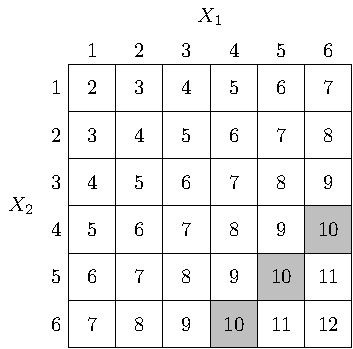
\includegraphics{math2750_files/figure-latex/dice-1} \end{center}

There are 3 possible ways to get \(Y=10\) (the grey cells in the table) out of the \(36\) possible outcomes, so we have \(\mathbb P(Y = 10) = 3/36 = 1/12\).

\end{myanswers}

\textbf{(b)} the conditional probability \(\mathbb P(Y=10 \mid X_1=x)\) for \(x=1, 2, \ldots, 6\);

\begin{myanswers}

\emph{Solution.} Conditioning on \(X_1 = x\) means restricting our attention only to column \(x\) of the table. Each column has \(6\) equally probably cells. For \(x=1,2,3\), none of the entries equal \(10\), so \(\mathbb P(Y=10 \mid X_1=x) = 0/6 = 0\). For each of \(x=4,5,6\), one of the entries equals \(10\), so \(\mathbb P(Y=10 \mid X_1=x) = 1/6\).

\end{myanswers}

\textbf{(c)} the conditional probability \(\mathbb P(X_1=x \mid Y=10)\) for \(x=1, 2, \ldots, 6\).

\begin{myanswers}

\emph{Solution.} Conditioning on \(Y =10\) means restricting our attention only to the \(3\) shaded cells, which are each equally likely. For \(x=1,2,3\), none of the shaded cells are in column \(x\), so \(\mathbb P(X_1=x \mid Y=10) = 0/3 = 0\). For each of \(x=4,5,6\), one of the shaded cells is in column \(x\), so \(\mathbb P(X_1=x \mid Y=10) = 1/3\).

\end{myanswers}

\textbf{3.} Let \((X_n)\) be a simple random walk starting from \(X_0 = 0\) and that at each step goes up one with probability \(p\) or down one with probability \(q = 1-p\). What are:

\textbf{(a)} \(\mathbb P(X_5 = 3)\),

\begin{myanswers}

\emph{Solution.} To get \(X_5 = 3\), we must take \(4\) steps up and \(1\) step down. The down step can be at any of the \(5\) time steps. Therefore we have \(\mathbb P(X_5 = 3) = 5p^4q\).

\end{myanswers}

\textbf{(b)} \(\mathbb P(X_5 = 3 \mid X_2 = 2)\),

\begin{myanswers}

\emph{Solution.} Once we're at \(X_2 = 2\), we must take \(2\) steps up and \(1\) step down over the next \(3\) time steps. So \(\mathbb P(X_5 = 3 \mid X_2 = 2) = 3p^2q\).

\end{myanswers}

\textbf{(c)} \(\mathbb P(X_n = n-2)\),

\begin{myanswers}

\emph{Solution.} This requires \(n-1\) steps up and \(1\) step down, and the down step can be at any of the \(n\) time steps. So \(\mathbb P(X_n = n-2) = np^{n-1}q\).

\end{myanswers}

\textbf{(d)} \(\mathbb E X_4\),

\begin{myanswers}

\emph{Solution.} The increments \(Z_n = X_n - X_{n-1}\) have expectation \(1p + (-1)q = p - q\), so \(\mathbb E X_4 = 4(p-q)\).

\end{myanswers}

\textbf{(e)} \(\mathbb E(X_6 \mid X_4 = 2)\),

\begin{myanswers}

\emph{Solution.} We are already at 2, then another two increments will take us up \(2(p-q)\) on average. Therefore \(\mathbb E(X_6 \mid X_4 = 2) = 2 + 2(p-q)\).

\end{myanswers}

\textbf{4.} The price \(X_n\) of a stock at the close of day \(n\) is modelled as a Gaussian random walk, where the increments \((Z_n)\) have a normal distribution \(Z_n \sim \text{N}(\mu, \sigma^2)\). The model assumes a drift of \(\mu = 0.7\) and a volatility of \(\sigma = 2.2\). The initial price is \(X_0 = 42.3\).

\textbf{(a)} Calculate the mean and variance of the price of the stock at the close of day \(5\).

\begin{myanswers}

\emph{Solution.} The mean and variance are
\begin{gather*}
  \mathbb EX_5 = \mathbb E X_0 + n \mathbb E Z_1 = 42.3 + 5 \cdot 0.7 = 45.8 , \\
  \operatorname{Var}X_5 = \operatorname{Var}X_0 + n \operatorname{Var}Z_1 = 0 + 5 (2.2)^2 = 24.2 .
  \end{gather*}

\end{myanswers}

\textbf{(b)} Give a 95\% prediction interval for the price at the close of day 5. (You might find it useful to recall that, if \(W \sim \text{N}(0,1)\) is a standard normal random variable, then \(\mathbb P(W \leq 1.96) = 0.975\).)

\begin{myanswers}

\emph{Solution.} Note that \(X_5\) itself is normally distributed, so \(X_5 \sim \text{N}(45.8,24.2)\). The 95\% prediction interval for a normal distribution \(\text{N}(\mu, \sigma^2)\) is \((\mu - 1.96\sigma, \mu + 1.96\sigma)\), so the prediction interval for \(X_5\) is
\[ \big(45.8 - 1.96\sqrt{24.2},  45.8 + 1.96\sqrt{24.2}\big) = (36.16, 55.44) . \]

\end{myanswers}

\textbf{(c)} After day 4, the prices at the end of each of the first four days have been recorded as \(X_1 = 44.4, X_2 = 44.0, X_3 = 47.1, X_4 = 47.8\). Update your prediction interval for the price at the close of day 5, and comment on how it differs from the earlier prediction interval.

\begin{myanswers}

\emph{Solution.} By the Markov property, \(X_5\) depends on \(X_4\), but given \(X_4\) does not depend on the other values, which we can therefore ignore. Since \(X_5 = X_4 + Z_5\), we have
\begin{gather*}
  \mathbb E(X_5 \mid X_4) = X_4 + \mathbb E Z_5 = 47.8 + 0.7 = 48.5 \\
  \operatorname{Var}(X_5 \mid X_4) = 0 + \operatorname{Var}Z_5 = 0 + (2.2)^2 = 4.84.
  \end{gather*}
The desired prediction interval is
\[ \big(48.5 - 1.96\sqrt{4.84},  48.5+ 1.96\sqrt{4.84}\big) = (44.19, 52.81) . \]
Compared to before, the centre of the prediction interval is slightly higher, because the stock has outperformed expectations so far, and the interval is much narrower, because as we get closer to day 5 we become less uncertain.

\end{myanswers}

\textbf{5.} A gambler decides to model her total winnings as a simple random walk starting from \(X_0 = 0\) that at each time goes up one with probability \(p\) and down one with probability \(1-p\), but where \(p\) is unknown. The first \(10\) recordings, \(X_1\) to \(X_{10}\), are
\[ (1, 2, 1, 2, 3, 4, 5, 6, 5, 6) . \]

\textbf{(a)} What would you guess for the value of \(p\), given this data?

\begin{myanswers}

\emph{Solution.} In \(10\) time steps, the process went up \(k = 8\) times and down \(n - k = 2\) times. So it seems reasonable to guess that \(p\) has the value \(\hat p = \frac{8}{10} = 0.8\).

\end{myanswers}

\textbf{(b)} More generally, how would you estimate \(p\) from the data \(X_0 = 0, X_1 = x_1, X_2 = x_2, \dots, X_n = x_n\)?

\begin{myanswers}

\emph{Solution.} We will estimate \(\hat p = k/n\), where \(k\) is the number of upward steps. We saw in lectures that \(k = (n + x_n)/2\), so our estimate is
\[ \hat p = \frac{n + x_n}{2n} = \frac12\ + \frac{x_n}{2n} . \]

\end{myanswers}

\textbf{(c)} Show that your estimate is in fact the maximum likelihood estimate of \(p\).

\begin{myanswers}

\emph{Solution.} The concept of ``maximum likelihood estimation'' will be known to those who have done MATH2715; this might be new for those who didn't take that course.

Let \(k = (n + x_n)/2\) be the number of upward steps. Then the ``likelihood'' is the probability mass function
\[ f(\mathbf x; p) = p^{k}(1-p)^{n-k} , \]
since we take \(k\) steps up and \(n-k\) steps down.
Given \(\mathbf x\) (or equivalently \(k\)) the ``maximum likelihood estimate'' is the value of \(p\) that maximises this likelihood.

As is often the case, it's equivalent but actually more convenient to maximise the log-likelihood
\[ \ell(\mathbf x; p) = \ln f(\mathbf x; p) = k \ln p + (n-k)\ln(1-p) .\]
We can perform the maximisation by differentiating and setting equal to \(0\). The derivative is
\[ \frac{\text{d}}{\text{d}p} \ell(\mathbf x; p) = \frac kp - \frac{n-k}{1-p} ,\]
so the maximum likelihood estimate \(\hat p\) satisfies
\[ 0 = \frac k{\hat p} - \frac{n-k}{1-\hat p} . \]

Solving this by clearing denominators we get
\[ 0 = (k - k\hat p) - (n\hat p - k\hat p) = k - n \hat p , \]
and rearranging gives \(\hat p = k/n\) as desired.

\end{myanswers}

\hypertarget{S03-gamblers-ruin}{%
\section{Gambler's ruin}\label{S03-gamblers-ruin}}

\begin{itemize}
\tightlist
\item
  The gambler's ruin Markov chain
\item
  Equations for probability of ruin and expected duration of the game by conditioning on the first step
\end{itemize}

\hypertarget{ruin-chain}{%
\subsection{Gambler's ruin Markov chain}\label{ruin-chain}}

Consider the following gambling problem. Alice is gambling against Bob. Alice starts with £\(a\) and Bob starts with £\(b\). It will be convenient to write \(m = a + b\) for the total amount of money, so Bob starts with £\((m-a)\). At each step of the game, both players bet £1; Alice wins £1 off Bob with probability \(p\), or Bob wins £1 off Alice with probability \(q\). The game continues until one player is out of money (or is ``ruined'').

Let \(X_n\) denote how much money Alice has after \(n\) steps of the game. We can write this as a stochastic process with discrete time \(n \in \{0,1,2,\dots\} = \mathbb Z_+\) and discrete state space \(\mathcal S = \{0,1,\dots,m\}\). Then \(X_0 = a\), and, for \(n \geq 0\), we have
\[ X_{n+1} = \begin{cases} X_n + 1 & \text{with probability $p$ if $1\leq X_n \leq m-1$,} \\
                           X_n - 1 & \text{with probability $q$ if $1\leq X_n \leq m-1$,} \\
                           0       & \text{if $X_n = 0$,} \\
                           m       & \text{if $X_n = m$.} \end{cases} \]
So Alice's money goes up one with probability \(p\) or down one with probability \(q\), unless the game is already over with \(X_n = 0\) (Alice is ruined) or \(X_n = m\) (Alice has won all Bob's money, so Bob in ruined).

We see that the gambler's ruin process \((X_n)\) clearly satisfies the Markov property: the next step \(X_{n+1}\) depends on where we are now \(X_n\), but, given that, does not depend on how we got here.

The gambler's ruin process is exactly like a simple random walk started from \(X_0 = a\) except that we have \textbf{absorbing barriers} and \(0\) and \(m\), where the random walk stops because one of the players has ruined. (One could also consider random walks with \textbf{reflecting barriers}, that bounce the random walk back into the state space, or \textbf{mixed barriers} that are absorbing or reflecting at random.)

There are two questions about the gambler's ruin that we'll try to answer in this section:

\begin{enumerate}
\def\labelenumi{\arabic{enumi}.}
\tightlist
\item
  What is the probability that the game ends by Alice ruining?
\item
  How long does the game last on average?
\end{enumerate}

\hypertarget{ruin-probability}{%
\subsection{Probability of ruin}\label{ruin-probability}}

The gambling game continues until either Alice is ruined (\(X_n = 0\)) or Bob is ruined (\(X_n = m\)). A natural question to ask is: What is the probability that the game ends in Alice's ruin?

Let us write \(r_i\) for the probability Alice ends up ruined if she currently has £\(i\). Then the probability of ruin for the whole game is \(r_a\), since Alice initially starts with £\(a\). The probability Bob will end up ruined is \(1 - r_a\), since one of the players must lose.

What can we say about \(r_i\)? Clearly we have \(r_0 = 1\), since \(X_n = 0\) means that Alice has run out of money and is ruined, and \(r_m = 0\), since \(X_n = m\) means that Alice has won all the money and Bob is ruined. What about when \(1 \leq i \leq m-1\)?

The key is to \emph{condition on the first step}. That is, we can write
\begin{align*}
\mathbb P(\text{ruin}) &= \mathbb P(\text{win first round}) \, \mathbb P(\text{ruin} \mid \text{win first round}) \\
&\qquad{}\quad {}+ \mathbb P(\text{lose first round}) \, \mathbb P(\text{ruin} \mid \text{lose first round}) \\
&= p\,\mathbb P(\text{ruin} \mid \text{win first round}) + q \,\mathbb P(\text{ruin} \mid \text{lose first round}) .
\end{align*}
Here we have conditioned on whether Alice wins or loses the first round. More formally, we have used the \textbf{law of total probability}, which says that if the events \(B_1, \dots, B_k\) are disjoint and cover the whole sample space, then
\[ \mathbb P(A) = \sum_{i=1}^k \mathbb P(B_i) \, \mathbb P(A \mid B_i) . \]
Here, \(\{\text{Alice wins the first round}\}\) and \(\{\text{Alice loses the first round}\}\) are indeed disjoint events that cover the whole sample space. This idea of ``conditioning on the first step'' will be the most crucial tool throughout this whole module.

If Alice wins the first round from having £\(i\), she now has £\((i+1)\). Her probability of ruin is now \(r_{i+1}\), because, by the Markov property, it's as if the game were starting again with Alice having £\((i+1)\) to start with. The Markov property tells us that it doesn't matter \emph{how} Alice got to having £\((i+1)\), it only matters how much she has now. Similarly, if Alice loses the first round, she now has £\((i-1)\), and the ruin probability is \(r_{i-1}\). Hence we have
\[ r_i = pr_{i+1} + qr_{i-1}. \]

Rearranging, and including the ``boundary conditions'', we see that the equation we want to solve is
\[ pr_{i+1} - r_i + qr_{i-1} = 0 \qquad \text{subject to} \qquad r_0 = 1,\ r_m = 0. \]
This is a \textbf{linear difference equation} -- and, because the left-hand side is \(0\), we call it a \textbf{homogeneous} linear difference equation.

We will see how to solve this equation in the next lecture. We will see that, if we set \(\rho = q/p\), then the ruin probability is given by
\[ r_a = \begin{cases} \displaystyle\frac{\rho^a - \rho^m}{1 - \rho^m} & \text{if $\rho \neq 1$,} \\[0.35cm]
           1 - \displaystyle\frac{a}{m} & \text{if $\rho = 1$.} \end{cases} \]
Note that \(\rho = 1\) is the same as the symmetric condition \(p = q = \frac12\).

Imagine Alice is not playing against a similar opponent Bob, but rather is up against a large casino. In this case, the casino's capital £\((m-a)\) is typically much bigger than Alice's £\(a\). We can model this by keeping \(a\) fixed taking a limit \(m \to \infty\). Typically, the casino has an ``edge'', meaning they have a better than \(50:50\) chance of winning; this means that \(q > p\), so \(\rho > 1\). In this case, we see that the ruin probability is
\[ \lim_{m \to \infty} r_a = \lim_{m \to \infty} \frac{\rho^a - \rho^m}{1 - \rho^m} = \lim_{m \to \infty} \frac{\rho^a/\rho^m - 1}{1/\rho^m - 1} = \frac{0-1}{0-1} = 1, \]
so Alice will be ruined with certainty.

Even with a generous casino that offered an exactly fair game with \(p = q = \frac12\), so \(\rho = 1\), we would have
\[ \lim_{m \to \infty} r_a = \lim_{m \to \infty}\left( 1 - \frac{a}{m} \right) = 1-0 = 1 , \]
so, even with this fair game, Alice would still be ruined with certainty.

(The official advice of the University of Leeds module MATH2750 is that you shouldn't gamble against a casino if you can't afford to lose.)

\hypertarget{expected-duration}{%
\subsection{Expected duration of the game}\label{expected-duration}}

We could also ask for how long we expect the game to last.

We approach this like before. Let \(d_i\) be the expected duration of the game from a point when Alice has £\(i\). Our boundary conditions are \(d_0 = d_m = 0\), because \(X_n = 0\) or \(X_n = m\) means that the game is over with Alice or Bob ruined. Again, we proceed by conditioning on the first step, so
\begin{align*}
\mathbb E(\text{duration}) &= \mathbb P(\text{win first round}) \, \mathbb E(\text{duration} \mid \text{win first round}) \\
&\qquad{}+ \mathbb P(\text{lose first round}) \, \mathbb E(\text{duration} \mid \text{lose first round}) \\
&= p\,\mathbb E(\text{duration} \mid \text{win first round}) + q \,\mathbb E(\text{duration} \mid \text{lose first round}) .
\end{align*}
More formally, we've used another version of the law of total probability,
\[ \mathbb E(X) = \sum_{i=1}^k \mathbb P(B_i) \, \mathbb E(X \mid B_i) , \]
or, alternatively, the \textbf{tower law} for expectations
\[ \mathbb E(X) = \mathbb E_Y \mathbb E (X \mid Y) = \sum_{y} \mathbb P(Y= y)\, E(X \mid Y = y), \]
where, in our case, \(Y\) was the outcome of the first round.

Now, the expected duration given we win the first round is \(1 + d_{i+1}\). This is because the round itself takes \(1\) time step, and then, by the Markov property, it's as if we are starting again from \(i+1\). Similarly, the expected duration given we lose the first round is \(1 + d_{i-1}\). Thus we have
\[ d_i = p(1 + d_{i+1}) + q (1 + d_{i-1}) = 1 + pd_{i+1} + qd_{i-1} . \]
Don't forget the 1 that counts the current round!

Rearranging, and including the boundary conditions, we have another linear difference equation:
\[ pd_{i+1} - d_i + qd_{i-1} = -1 \qquad \text{subject to} \qquad d_0 = 0,\ d_m = 0. \]
Because the right-hand side, \(-1\), is nonzero, we call this an \textbf{inhomogeneous} linear difference equation.

Again, we'll see how to solve this in the next lecture, and will find that the solution is given by
\[ d_a = \begin{cases} {\displaystyle \frac{1}{q-p} \left(a - m\frac{1-\rho^a}{1- \rho^m} \right)} & \text{if $\rho \neq 1$,} \\
\displaystyle a(m-a) & \text{if $\rho = 1$.} \end{cases} \]

Thinking again of playing against the casino, with \(q > p\), \(\rho > 1\), and \(m \to \infty\), we see that the expected duration is
\[ \lim_{m\to\infty} d_a = \lim_{m\to\infty} \frac{1}{q-p} \left(a - m\frac{1-\rho^a}{1 - \rho^m} \right)  = \frac{1}{q-p} \left(a - 0 \right) = \frac{a}{q-p} , \]
since \(\rho^m\) grows much quicker than \(m\). So Alice ruins with certainty, and it will take time \(a/(q-p)\), on average.

In the case of the generous casino, though, with \(q = p\), so \(\rho = 1\), we have
\[ \lim_{m\to\infty} d_a =  \lim_{m\to\infty} a(m-a) = \infty .  \]
So here, Alice will ruin with certainty, but it may take a very long time until the ruin occurs, since the expected duration is infinite.

\textbf{In the next section}, we see how to solve linear difference equations, in order to find the ruin probability and expected duration of the gambler's ruin.

\hypertarget{S04-ldes}{%
\section{Linear difference equations}\label{S04-ldes}}

\begin{itemize}
\tightlist
\item
  How to solve homogeneous and inhomogeneous linear difference equations
\item
  Solving for probability of ruin and expected duration of the gambler's ruin
\end{itemize}

In \protect\hyperlink{S03-gamblers-ruin}{the previous section}, we looked at the probability of ruin and expected duration of the gambler's ruin process. We set up linear difference equations to find these. In this section, we'll learn how to solve these equations.

A \textbf{linear difference equation} is an equation that looks like
\begin{equation}
a_k x_{n+k} + a_{k-1} x_{n+k-1} + \cdots + a_1 x_{n+1} + a_0 x_n = f(n) \label{eq:lde} 
\end{equation}
for \(n = 0,1,\dots\), where the \(a_i\) are given constants, \(f(n)\) is a given function, and we want to solve for the sequence \((x_n)\). The equation normally comes with some extra conditions, such as the value of the first few \(x_n\)s.

When the right-hand side of \eqref{eq:lde} is zero, so \(f(n) = 0\), we say the equation is \textbf{homogeneous}; when the right-hand side is nonzero, it is \textbf{inhomogeneous}. The number \(k\), where there are \(k+1\) terms on the left-hand side, is called the \textbf{degree} of the equation; we are mostly interested in second-degree linear difference equations, which have three terms on the left-hand side.

\hypertarget{hom-ldes}{%
\subsection{Homogeneous linear difference equations}\label{hom-ldes}}

We start with the homogeneous case, which is simpler.

Consider a homogeneous linear difference equation. We shall use the second-degree example
\[ x_{n+2} - 5x_{n+1} + 6x_{n} = 0 \qquad \text{subject to } x_0 = 4, x_1 = 9 .  \]
Here, the conditions on \(x_0\) and \(x_1\) are \textbf{initial conditions}, because they tell us how the sequence \((x_n)\) starts.

For the moment, we shall put the initial conditions to the side and just worry about the equation
\[ x_{n+2} - 5x_{n+1} + 6x_{n} = 0 . \]
We start by guessing there might be a solution of the form \(x_n = \lambda^n\) for some constant \(\lambda\). We can find out if there is such a solution by substituting in \(x_n = \lambda^n\), and seeing if there's a \(\lambda\) that solves the equation. For our example, we get
\[ \lambda^{n+2} - 5 \lambda^{n+1} + 6\lambda^n = 0 . \]
After cancelling off a common factor of \(\lambda^n\), we get
\[ \lambda^2 - 5 \lambda + 6 = 0 . \]
This is called the \textbf{characteristic equation}. For a general homogeneous linear difference equation \eqref{eq:lde}, the characteristic equation is
\begin{equation}
  a_k \lambda^{k} + a_{k-1} \lambda^{k-1} + \cdots + a_1 \lambda + a_0 = 0 .  \label{eq:cheq} 
\end{equation}
When writing out answers to questions, you can jump straight to the characteristic equation.

We can now solve the characteristic equation for \(\lambda\). In our example, we can factor the left-hand side to get \((\lambda - 3)(\lambda - 2) = 0\), which has solutions \(\lambda = 2\) and \(\lambda = 3\). Thus \(x_n = 2^n\) and \(x_n = 3^n\) both solve our equation. In fact, since the right-hand side of the equation is \(0\), any linear combination of these two solutions is a solution also, thus we get the \textbf{general solution}
\[ x_n = A 2^n + B 3^n , \]
which is a solution for any values of the constants \(A\) and \(B\).

For a general characteristic equation with distinct roots \(\lambda_1, \lambda_2, \dots, \lambda_k\), the general solution is
\[ x_n = C_1 \lambda_1^n + C_2 \lambda_2^n + \cdots + C_k \lambda_k^n . \]
If we have a repeated root -- say, \(\lambda_1 = \lambda_2 = \cdots = \lambda_r\) is repeated \(r\) times -- than you can check that a solution is given by
\[ x_n = (D_0 + D_1 n + \cdots + D_{r-1} n^{r-1}) \lambda_1^n , \]
which should take its place in the general solution.

Once we have the general solution, we can use the extra conditions to find the values of the constants. In our example, we can use the initial conditions to find out the values of \(A\) and \(B\). We see that
\begin{gather*}
x_0 = A2^0 + B3^0 = A + B = 4 , \\
x_1 = A2^1 + B3^1 = 2A + 3B = 9 .
\end{gather*}
We can now solve this pair of simultaneous equations to solve for \(A\) and \(B\). By subtracting twice the first equation from the second we get \(B = 1\), and substituting this into the first equation we get \(A = 3\). Thus the solution is
\[ x_n = 3\cdot 2^n + 3^n . \]

In conclusion, the process here was:

\begin{enumerate}
\def\labelenumi{\arabic{enumi}.}
\tightlist
\item
  Find the general solution by writing down and solving the characteristic equation.
\item
  Use the extra conditions to find the values of the constants in the general solution.
\end{enumerate}

Here are two more examples. These also give an idea of how I would expect you to set out your own answers to similar problems.

\begin{example}
\protect\hypertarget{exm:lde1}{}\label{exm:lde1}

\emph{Solve the homogeneous linear difference equation}
\[ x_{n+2} - x_{n+1} - 6x_n = 0 \qquad \text{subject to} \quad x_0 = 3,\quad x_1 = 4 . \]

\emph{Step 1.} The characteristic equation is
\[ \lambda^2 - \lambda - 6 = 0 . \]
We can solve this by factorising it as \((\lambda - 3) (\lambda + 2) = 0\),
to find the solutions \(\lambda_1 = -2\) and \(\lambda_2 = 3\). Thus the general solution is
\[ x_n = A(-2)^n + B3^n . \]

\emph{Step 2.} Substituting the initial conditions into the general solution, we have
\begin{align*}
x_0 &= A(-2)^0 + B3^0 = A + B = 3 \\
x_1 &= A(-2)^1 + B3^1 = -2A + 3B = 4 .
\end{align*}
We can add twice the first equation to the second to get \(5B = 10\), so \(B=2\). We can substitute this into the first equation to get \(A = 1\).

The solution is therefore
\[ x_n = 1\cdot(-2)^n + 2 \cdot 3^n = (-2)^n + 2 \cdot 3^n . \]

\end{example}

\begin{example}
\protect\hypertarget{exm:lde2}{}\label{exm:lde2}

\emph{Solve the homogeneous linear difference equation}
\[ x_{n+2} + 4x_{n+1} +4x_n = 0 \qquad \text{subject to} \quad x_0 = 2,\quad x_1 = -6 . \]

\emph{Step 1.} The characteristic equation is
\[ \lambda^2 + 4\lambda + 4 = 0 . \]
We can solve this by factorising it as \((\lambda + 2)^2 = 0\), to find a repeated root \(\lambda_1 = \lambda_2 = -2\). Thus the general solution is
\[ x_n = (A + Bn) (-2)^n . \]

\emph{Step 2.} Substituting the initial conditions into the general solution, we have
\begin{align*}
x_0 &= (A + B0)(-2)^0 = A = 2 \\
x_1 &= (A + B1)(-2)^1 = -2A - 2B = -6 .
\end{align*}
The first immediately gives \(A = 2\), and substituting this into the second equation gives \(B = 1\).

The solution is therefore
\[ x_n = (2 + n)(-2)^n . \]

\end{example}

\hypertarget{ruin-probability-solve}{%
\subsection{Probability of ruin for the gambler's ruin}\label{ruin-probability-solve}}

In the last lecture we saw that probability of ruin for the gambler's ruin process is the solution to
\[ pr_{i+1} - r_i + qr_{i-1} = 0 \qquad \text{subject to} \qquad r_0 = 1,\ r_m = 0 , \]
where the extra conditions here are \textbf{boundary conditions}, because they tell us what happens at the boundaries of the state space.

The characteristic equation is
\[ p\lambda^2 - \lambda + q = 0 .\]
We can solve the characteristic equation by factorising it as \((p \lambda - q)(\lambda - 1) = 0\). (It might take a moment to check this really is a factorisation of the characteristic equation. Hint: we've used that \(p+q=1\).) So the characteristic equation has roots \(\lambda = q/p\), which we called \(\rho\) last time, and \(\lambda = 1\). Now, if \(\rho = 1\) (so \(p = q = \frac12\)) we have a repeated root, while if \(\rho \neq 1\) we have distinct roots, so we'll need to deal with the two cases separately.

First, the case \(\rho \neq 1\). Since the two roots are distinct, we have the general solution
\[ r_i = A\rho^i + B1^i = A\rho^i + B . \]

We can now use the boundary conditions to find \(A\) and \(B\). We have
\begin{gather*} r_0 = A \rho^0 + B = A+B = 1, \\
                r_m = A \rho^m + B = 0 . \end{gather*}
From the first we get \(B = 1-A\), which we substitute into the second to get
\[ A\rho^m + 1 - A = 0 \quad \Rightarrow \quad A = \frac{1}{1-\rho^m} , \]
and hence
\[ B = 1 - A = 1 - \frac{1}{1-\rho^m} = - \frac{\rho^m}{1 - \rho^m} . \]
Thus the solution is
\[ r_i = \frac{1}{1-\rho^m} \rho^i -  \frac{\rho^m}{1 - \rho^m} = \frac{\rho^i - \rho^m}{1 - \rho^m}  , \]
as we claimed last time.

Second, the case \(\rho = 1\). Now we have a repeated root \(\lambda = 1\), so the general solution is
\[ r_i = (A + Bi) 1^i = A+Bi . \]

Again, we use the boundary conditions, to get
\begin{gather*} r_0 = A + B\cdot 0 = A = 1, \\
r_m = A + Bm = 0 , \end{gather*}
and we immediately see that \(A = 1\) and \(B = -1/m\). Thus the solution is
\[ r_i = 1 - \frac{1}{m}i = 1 - \frac{i}{m} , \]
as claimed last time.

\hypertarget{inhom-ldes}{%
\subsection{Inhomogeneous linear difference equations}\label{inhom-ldes}}

Solving inhomogeneous linear difference equations requires three steps:

\begin{enumerate}
\def\labelenumi{\arabic{enumi}.}
\tightlist
\item
  Find the general solution to the \emph{homogeneous} equation by writing down and solving the characteristic equation.
\item
  By making an ``educated guess'', find a solution (a ``particular solution'') to the inhomogeneous equation. The general solution to the inhomogeneous equation is a particular solution plus the general solution to the homogeneous equation.
\item
  Use the extra conditions to find the values of the constants in the general solution.
\end{enumerate}

This idea works because, once you have a particular solution, adding a solution to the \emph{homogeneous} equation to the left-hand side adds zero to the right-hand side, so maintains a solution to the inhomogeneous equation.

Let's work through the example
\[ x_{n+2} - 5x_{n+1} + 6x_{n} = 2 \qquad \text{subject to } x_0 = 4, x_1 = 9 . \]

We already know from earlier that the general solution to the homogeneous equation \(x_{n+2} - 5x_{n+1} + 6x_{n} = 0\) (with a zero on the right-hand side) is
\[ x_n = A2^n + B3^n . \]

We now need to find a \textbf{particular solution} -- that is, any solution -- to our new inhomogeneous equation. The usual process here is to guess a solution with the same ``shape'' as the right-hand side. For example, if the right-hand side is a constant, try a constant for the particular solution. Here our right-hand side is the constant \(2\), so we should try a constant \(x_n = C\). Substituting this into the inhomogeneous equation gives us \(C - 5C + 6C = 2\), thus \(2C = 2\) and \(C = 1\), giving a particular solution \(x_n = 1\). The general solution to the inhomogeneous equation is therefore
\[ x_n = 1 + A2^n + B3^n , \]
the sum of the particular solution \(x_n = 1\) and the general solution to the homogeneous equation.

Because the right-hand side was a constant, we guessed a constant -- this is the main case we will deal with. Other cases you could come across include:

\begin{itemize}
\tightlist
\item
  If the right-hand side is a polynomial of degree \(d\), try a polynomial of degree \(d\).
\item
  If the right-hand side is \(\alpha^n\) for some \(\alpha\), try \(C\alpha^n\).
\item
  If the right-hand side is a constant, but a constant \(C\) doesn't work, try \(Cn\). If that still doesn't work, try \(Cn^2\), and so on. A general rule is that is 1 is a root of the characteristic equation with multiplicity \(m\), you need to try \(Cn^m\). We discuss this case further in the next subsection.
\end{itemize}

Continuing with the example, we use the initial conditions to get the constants \(A\) and \(B\). We have
\begin{gather*}
x_0 = 1 + A2^0 + B3^0 = 1+ A + B = 4 , \\
x_1 = 1 + A2^1 + B3^1 = 1+ 2A + 3B = 9 .
\end{gather*}
The second equation minus twice the first gives \(-1 + B = 1\), so \(B=2\), and substituting that back into the first gives \(A = 1\). Thus the solution is
\[ x_n = 1 + 1\cdot 2^n + 2 \cdot 3^n = 1 + 2^n + 2 \cdot 3^n . \]

Here's another example.

\begin{example}
\protect\hypertarget{exm:lde3}{}\label{exm:lde3}

\emph{Solve the inhomogeneous linear difference equation}
\[ 10 x_{n+2} - 7x_{n+1} + x_n = 8 \qquad \text{subject to} \quad x_0 = 0,\quad x_1 = \tfrac{13}{10} . \]

\emph{Step 1.} The characteristic equation is
\[ 10\lambda^2 - 7\lambda + 1 = 0 . \]
We can solve this by factorising it as
\[ (2\lambda - 1) (5\lambda - 1) = 0 , \]
to find the solutions \(\lambda_1 = \frac12\) and \(\lambda_2 = \frac15\). Thus the general solution of the homogeneous equation is
\[ x_n = A\left(\frac12\right)^n + B\left(\frac15\right)^n . \]

\emph{Step 2.} Since the right hand side of the inhomogeneous equation is a constant, we guess a constant particular solution with shape \(x_n = C\). Substituting in this guess, we get
\[ 10C - 7C + C = 4C = 8 \]
with solution \(C=2\). Thus a particular solution is \(x_n = 2\), and the general solution to the inhomogeneous equation is
\[ x_n = 2 + A\left(\frac12\right)^n + B\left(\frac15\right)^n . \]

\emph{Step 3.} Substituting the initial conditions into the general solution, we have
\begin{align*}
x_0 = 2 + A\left(\frac12\right)^0 + B\left(\frac15\right)^0 = 2 + A + B = 0 \quad &\Rightarrow \quad A + B = -2 \\
x_1 = 2 + A\left(\frac12\right)^1 + B\left(\frac15\right)^1 = 2 + A\frac12 + B\frac15 = \frac{13}{10} \quad &\Rightarrow \quad 5A + 2B = -7.
\end{align*}
We can take twice the first equation abd subtract the second to get \(-3A = 3\), so \(A = -1\). We can substitute this into the second equation to get \(B = -1\).

The solution is therefore
\[ x_n = 2 - \left(\frac12\right)^n - \left(\frac15\right)^n . \]

\end{example}

\hypertarget{duration-solve}{%
\subsection{Expected duration for the gambler's ruin}\label{duration-solve}}

From last time, the expected duration of the gambler's ruin game solves
\[ pd_{i+1} - d_i + qd_{i-1} = -1 \qquad \text{subject to} \qquad d_0 = 0,\ d_m = 0. \]
As before, we divide cases based on whether or not \(\rho = 1\).

First, the case \(\rho \neq 1\). We already know that the general solution to the homogeneous equation is
\[ d_i =  A \rho^i + B . \]

Now we need a particular solution. It's tempting to guess a constant \(C\) for a particular solution, but we know that constants solve the homogeneous equation, since \(d_i = B\) is a solution, so a constant will give right-hand side \(0\), not \(-1\). (We could try out \(x_i = C\) if we wanted; we would get \((p - 1 + q)C = -1\), but \(p-1+q=0\), and \(0 \times C = -1\) has no solution.) The next best try is to go one degree up: let's guess \(x_i = Ci\) instead. This gives
\begin{align*}
  -1 &= pC(i+1) - Ci + qC(i-1)\\
     &= C(pi + p - i + qi - q) \\
     &= C\big((p+q-1)i + (p-q)\big) \\
     &= C(p-q) ,
  \end{align*}
since \(p + q - 1 = 1 - 1 = 0\). This \(C = -1/(p-q) = 1/(q-p)\). Finding a solution for \(C\) shows that our guess worked. The general solution to the inhomogeneous equation is
\[ d_i = \frac{i}{q-p} + A \rho^i + B .  \]

Then to find the constants, we have
\begin{gather*} d_0 = \frac{0}{q-p} + A \rho^0 + B = A+B = 0, \\
                  d_m = \frac{m}{q-p} + A \rho^m + B = 0 , \end{gather*}
which you can check gives
\[ A = -B = \frac{m}{q-p} \cdot \frac{1}{1 - \rho^m} . \]
Hence, the solution is
\[ d_i = \frac{i}{q-p} + \frac{m}{q-p} \frac{1}{1 - \rho^m} \rho^i - \frac{m}{q-p} \frac{1}{1 - \rho^m} =  \frac{1}{q-p} \left(i - m\frac{1-\rho^i}{1- \rho^m} \right) . \]

Second, the case \(\rho = 1\), so \(p = q = \frac12\). We already know that the general solution to the homogeneous equation is
\[ d_i =  A + Bi . \]

We need a particular solution. Since 1 is a double root of the characteristic equation, both constants \(x_i = A\) and linear \(x_i = Bi\) terms solve the homogeneous equation. (You can check that guessing \(x_i = C\) or \(x_i = Ci\) doesn't work, if you like.) So we'll have to go up another degree and try \(x_i = Ci^2\). This gives
\begin{align*}
    -1 &= \tfrac12 C(i+1)^2 - Ci^2 + \tfrac 12 C(i-1)^2 \\
       &= \tfrac12 C(i^2 + 2i + 1 - 2i^2 + i^2 - 2i + 1) \\
       &= \tfrac12 C\big((1-2+1)i^2 + (2-2)i + (1+1)\big) \\
       &=C ,
\end{align*}
so the general solution to the inhomogeneous equation is
\[ d_i = -i^2 + A + Bi .  \]

Then to find the constants, we have
\begin{gather*} d_0 = -0^2 + A + B\cdot0 = A = 0, \\
                  d_m = -m^2 + A + Bm = 0 , \end{gather*}
giving \(A = 0, B = m\). The solution is
\[ d_i = -i^2 + 0 + mi = i(m-i) .\]

\textbf{In the next section}, we move on from the specific cases we've looked at so far to the general theory of discrete time Markov chains.

\hypertarget{P02}{%
\section*{Problem sheet 2}\label{P02}}
\addcontentsline{toc}{section}{Problem sheet 2}

\commtrue

You should attempt all these questions and write up your solutions in advance of your workshop in week 3 (Monday 8 or Tuesday 9 February) where the answers will be discussed.

\textbf{1.} Solve the following linear difference equations:

\textbf{(a)} \(x_{n+2} - 4x_{n+1} + 3x_{n} = 0\), subject to \(x_0 = 0\), \(x_1 = 2\).

\begin{myanswers}

\emph{Solution.} The characteristic equation is \(\lambda^2 - 4\lambda + 3 = 0\), which factorises as \((\lambda - 3)(\lambda - 1) = 0\), with solutions \(\lambda = 1,3\), so the general solution is \(x_n = A1^n + B3^n = A + B3^n\). The initial conditions give \(A+B = 0\) and \(A + 3B = 2\), meaning \(B = 1\) and \(A = -1\). Hence the solution is \(x_n = 3^n - 1\).

\end{myanswers}

\textbf{(b)} \(4x_{n+1} = 4x_n - x_{n-1}\), subject to \(x_0 = 1\), \(x_1 = 0\).

\begin{myanswers}

\emph{Solution.} First, we rearrange to \(4x_{n+1} - 4x_n + x_{n-1} = 0\). The characteristic equation is \(4\lambda^2 - 4\lambda + 1 = 0\), which factorises as \((2\lambda - 1)^2 = 0\), which has a repeated root \(\lambda = \frac12\), so the general solution is \(x_n = (A + Bn)(\frac12)^n\). The initial conditions give \(A=1\) and \((A + B)/2 = 0\), meaning \(B = -1\). Hence the solution is \(x_n = (1 - n)(\frac12)^n\).

\end{myanswers}

\textbf{(c)} \(x_n-5x_{n-1} + 6x_{n-2} = 1\), subject to \(x_0 = 1\), \(x_1 = 2\).

\begin{myanswers}

\emph{Solution.} The characteristic equation is \(\lambda^2 - 5\lambda + 6 = 0\), which factorises as \((\lambda - 2)(\lambda - 3) = 0\), with solutions \(\lambda = 2,3\), so the general solution to the homogeneous equation is \(A2^n + B3^n\). For a particular solution, we guess a solution of the form \(x_n = C\); substituting this into the inhomogeneous equation gives \(C - 5C + 6C = 1\), so \(C = \frac12\). So the general solution to the inhomogeneous equation is \(x_n = A2^n + B3^n + \frac12\). The initial conditions give \(A+B \frac12= 1\) and \(2A + 3B + \frac12= 2\), which is solved by \(B = \frac12\) and \(A = 0\). Hence the solution is \(x_n = \frac12 3^n + \frac12 = (3^n + 1)/2\).

\end{myanswers}

\textbf{(d)} \(x_{n+2} - 2x_{n+1} + x_n = -1\), subject to \(x_0 = 0\), \(x_1 = 2\).

\begin{myanswers}

\emph{Solution.} The characteristic equation is \(\lambda^2 - 2\lambda + 1 = 0\), which factorises as \((\lambda - 1)^2 = 0\), with a repeated root \(\lambda = 1\), so the general solution to the homogeneous equation is \((A + Bn)1^n = A + Bn\). For a particular solution, since constant and linear terms will equal \(0\), not \(-1\), we guess a solution of the form \(x_n = Cn^2\); substituting this into the inhomogeneous equation gives
\[ C(n+2)^2 - 2C(n+1)^2 + Cn^2 = 2C = -1  \]
so \(C = -\frac12\). So the general solution to the inhomogeneous equation is \(x_n = A + Bn - \frac12 n^2\). The initial conditions give \(A = 0\) and \(A + B - \frac12= 2\), so \(B = \frac52\). Hence the solution is \(x_n = \frac52n - \frac12n^2 = \frac n2(5-n)\).

\end{myanswers}

\textbf{2.} Consider a simple symmetric random walk on the state space \(\mathcal{S} = \{0,1,\ldots ,m\}\) with an absorbing barrier at \(0\) and a reflecting barrier at \(m\). In other words,
\[ \mathbb P(X_{n+1} = 0 \mid X_n = 0) = 1 \quad \text{and} \quad  \mathbb P(X_{n+1} = m-1 \mid X_n = m) = 1 . \]
Let \(\eta_i\) be the expected time until the the walk hits \(0\) when starting from \(i \in \mathcal S\).

\textbf{(a)} Explain why \((\eta_i)\) satisfies
\[ \eta_i = 1 + \tfrac12 \eta_{i+1} +\tfrac12 \eta_{i-1} \]
for \(i \in \{1,2,\dots,m-1\}\).

\begin{myanswers}

\emph{Solution.} We condition on the first step. The first step itself takes time 1. After that, with probability \(\frac12\) we are at state \(i+1\), with expected time remaining \(\eta_{i+1}\), while with probability \(\frac12\) we are at state \(i-1\), with expected time remaining \(\eta_{i-1}\).

\end{myanswers}

\textbf{(b)} Give a similar equation for \(\eta_m\), and state the value of \(\eta_0\).

\begin{myanswers}

\emph{Solution.} From \(m\), we move to \(m-1\) with certainty, so conditioning on the first step gives \(\eta_m = 1 + \eta_{m-1}\).

Clearly \(\eta_0 = 0\), as we stop immediately.

\end{myanswers}

\textbf{(c)} Hence, find the value of \(\eta_i\) for all \(i \in \mathcal S\).

\begin{myanswers}

\emph{Solution.} We rewrite the equation as \(\eta_{i+1} - 2 \eta_i + \eta_{i-1} = -2\). This has characteristic equation \(\lambda^2 - 2\lambda + 1 = 0\), which factorises as \((\lambda-1)^2\), with a repeated root of \(1\), so the general solution to the homogeneous equation is \(A + Bi\). By the same logic as before, we attempt a particular solution of the form \(\eta_i = Ci^2\), which gives
\[ C(i+1)^2 - 2Ci^2 + C(i-1)^2 = 2C = -2 ,   \]
so \(C = -1\). The general solution to the inhomogeneous equation is therefore \(\eta_i = A + Bi - i^2\). From the boundary condition \(k_0 = 0\) we have \(A = 0\). From the boundary condition \(k_m = 1 + k_{m-1}\) we have
\[ Bm - m^2 = 1 + B(m-1) - (m-1)^2 = Bm - B - m^2 +2m  , \]
giving \(B = 2m\). Therefore the solution is \(\eta_i = 2mi - i^2 = i(2m - i)\).

\end{myanswers}

\textbf{(d)} You should notice that your answer is the same as the expected duration of the gambler's ruin for \(p = \frac12\), except with \(m\) replaced by \(2m\). Can you explain why this might be?

\begin{myanswers}

\emph{Solution.} This is an example of the \textbf{reflection principle}. Let \((Y_n)\) be a gambler's ruin (simple random walk with two absorbing barriers) on \(\{0,1,\dots, 2m\}\). Then consider placing a mirror at \(m\), and viewing the Markov chain so that it remains in the first half \(\{0,1,\dots,m\}\); more formally, we consider \((X_n)\) where
\[ X_n = \begin{cases} Y_n & \text{if $Y_n \leq m$} \\
                      2m - Y_n & \text{if $Y_n > m$.} \end{cases}   \]
Then \((X_n)\) is the half-reflecting random walk we consider in this question. Further, \((X_n)\) is absorbed at \(0\) when \((Y_n)\) is absorbed at either \(0\) or \(2m\), which has the given expected time \(i(2m-i)\).

\end{myanswers}

\textbf{3.} Consider the gambler's ruin problem with draws: at each step, Alice wins £1 with probability \(p\), loses £1 with probability \(q\), and neither wins nor loses any money with probability \(s\), where \(p + q +s = 1\), and \(0 < p,q,s<1\). Alice starts with £\(a\) and Bob with £\((m-a)\).

\textbf{(a)} Let \(r_i\) be Alice's probability of ruin given that she has £\(i\).

\textbf{(i)} Write down a linear difference equation for \((r_i)\), remembering to include appropriate boundary conditions.

\begin{myanswers}

\emph{Solution.} By conditioning on the first step, we have
\[ r_i = pr_{i+1} + sr_i + qr_{i-1} , \]
which can be rearranged to
\[ pr_{i+1} - (1-s)r_i + qr_{i-1} = 0 . \]
The boundary conditions are \(r_0 = 1\) and \(r_m = 0\).

\end{myanswers}

\textbf{(ii)} Solve the linear difference equation, to find \(r_a\), Alice's probability of ruin. You may assume that \(p \neq q\).

\begin{myanswers}

\emph{Solution.} The characteristic equation is \(p\lambda^2 - (1-s)\lambda + q = 0\), which factorises as \((p\lambda - q)(\lambda - 1) = 0\), since \(p + q = 1-s\). The solutions are \(\lambda = q/p = \rho\) and \(\lambda = 1\). Since we assume \(p \neq q\), we have that \(\rho \neq 1\), so we have unique roots, and general solution
\(r_i = A + B \rho^i\). The boundary conditions give \(A + B = 1\) and \(A + B\rho^m = 0\), meaning that \(B = 1/(1-\rho^m)\) and \(A = -\rho^m/(1-\rho^m)\), so the solution is
\[ r_i = -\frac{\rho^m}{1-\rho^m} + \frac{1}{1-\rho^m}\rho^i = \frac{\rho^i - \rho^m}{1-\rho^m}.   \]

\end{myanswers}

\textbf{(b)} Let \(d_i\) be be the expected duration of the game from the point that Alice has £\(i\).

\textbf{(i)} Write down a linear difference equation for \((d_i)\), remembering to include appropriate boundary conditions.

\begin{myanswers}

\emph{Solution.} By conditioning on the first step, we have
\[ d_i = p(1 + d_{i+1}) + s(1 + d_i) + q(1 + d_{i-1}) ,  \]
which after rearranging gives
\[ pd_{i+1} - (1-s)d_i + qd_{i-1} = -1.  \]
The boundary conditions are \(d_0 = 0\) and \(d_m = 0\).

\end{myanswers}

\textbf{(ii)} Solve the linear difference equation, to find \(d_a\), the expected duration of the game. You may assume that \(p \neq q\).

\begin{myanswers}

\emph{Solution.} As before, the solution to the homogeneous equation is \(A + B\rho^i\). We try a particular solution of the for \(d_i = Ci\), and find that
\[ pC(i+1) -(1-s)Ci + qC(i-1) = C(p-q) = -1 ,\]
so \(C= 1/(q-p)\), and the general solution to the inhomogeneous equation is
\[ d_i = A + B\rho^i + \frac{i}{q-p} .  \]
The boundary conditions give \(A + B = 0\) and \(A + B \rho^m + m/(q-p) = 0\), meaning that
\[ B = -A = \frac{m}{q-p} \frac{1}{1-\rho^m} . \]
Hence the solution is
\[ d_i = \frac{1}{q-p} \left(i - m\frac{1-\rho^i}{1-\rho^m} \right) .   \]

\end{myanswers}

\textbf{(c)} Alice starts playing against Bob in a standard gambler's ruin game with probabilities \(p \neq q\) and \(s = 0\). A draw probability \(s > 0\) is then introduced in such a way that the ratio \(\rho = q/p\) remains constant. Comment on how this changes Alice's ruin probability and the expected duration of the game.

\begin{myanswers}

\emph{Solution.} The ruin probability does not change, as we see immediately. This is not surprising, as the win and lose probabilities for a round conditional on the round not being a draw have stayed the same.

The expected duration of the game increases. If \(\rho = q/p\) stays the same while introducing a draw probability \(s\), then the ``new'' \(q\) and \(p\) are \((1-s)q\) and \((1-s)p\), so \(q-p\) becomes\((1-s)q - (1-s)p = (1-s)(q-p)\). Hence expected duration goes up by a factor of \(1/(1-s)\). This makes sense, since number of rounds until a non-draw result is a geometric distribution with expectation \(1/(1-s)\), so each step takes \(1/(1-s)\) times as long on average.

\end{myanswers}

\textbf{4.} The Fibonacci numbers are 1, 1, 2, 3, 5, 8, 13, 21, 34, \ldots, where each number in the sequence is the sum of the two previous numbers. Show that the ratio of consecutive Fibonacci numbers tends to the ``golden ratio'' \(\phi = (1 + \sqrt{5})/2\).

\begin{myanswers}

\emph{Solution.} The Fibonacci numbers \((F_n)\) satisfy \(F_{n+1} = F_n + F_{n-1}\), which rearranges to \(F_{n+1} -F_n - F_{n-1} = 0\). The is a linear difference equation with characteristic equation \(\lambda^2 - \lambda - 1 = 0\). This has two solutions, which can be found using the quadratic formula. The solution with larger absolute value is \(\lambda_1 = (1+\sqrt{5})/2 = \phi\), the golden ratio, and the solution with smaller absolute value is \(\lambda_2 = (1-\sqrt{5})/2\). Hence, the general solution to the equation is \(F_n = A\phi^n + B\lambda_2^n\). We could use the initial conditions \(F_1 = 1\) and \(F_2 = 1\) to find \(A\) and \(B\), but there's no need to here.

The ratio of consecutive Fibonacci numbers is
\[ \frac{F_{n+1}}{F_n} = \frac{A\phi^{n+1} + B\lambda_2^{n+1}}{A\phi^n + B\lambda_2^n} = \frac{\phi + B\lambda_2^{n+1}/A\phi^n}{1 + B\lambda_2^n/A\phi^n} \to \frac{\phi + 0}{1 + 0} = \phi \]
as \(n \to \infty\), since \(|\lambda_2/\phi| < 1\) means that \(\lambda_2^n / \phi^n \to 0\).

\end{myanswers}

\hypertarget{A1}{%
\section*{Assessment 1}\label{A1}}
\addcontentsline{toc}{section}{Assessment 1}

This assessment counts as 4\% of your final module grade. You should attempt both questions. You must show your working, and there are marks for the quality of your mathematical writing.

The deadline for submission is \textbf{Thursday 11 February at 2pm}. Submission will be to Gradescope via Minerva, from Monday 8 February. It would be helpful to start your solution to Question 2 on a new page. If you hand-write your solutions and scan them using your phone, please convert to PDF using a scanning app (I like Microsoft Office Lens or Adobe Scan) rather than submit images.

Late submissions up to Wednesday 17 February at 2pm will still be marked, but the total mark will be reduced by 10\% per day or part-day for which the work is late. Submissions are not permitted after Wednesday 17 February.

Your solutions to this assessment should be your own work. Copying, collaboration or plagiarism are not permitted. Asking others to do your work, including via the internet, is not permitted. Transgressions are considered to be a very serious matter, and will be dealt with according to the University's disciplinary procedures.

\textbf{1.} Let \((X_n)\) be a simple random walk that starts from \(X_0 = 0\) and on each step goes up one with probability \(p\) and down one with probability \(q = 1-p\).

Calculate:

\textbf{(a)} \(\mathbb P(X_6 = 0)\), {{[}1 mark{]}}

\textbf{(b)} \(\mathbb EX_6\), {{[}1{]}}

\textbf{(c)} \(\text{Var}(X_6)\), {{[}1{]}}

\textbf{(d)} \(\mathbb E(X_{10} \mid X_4 = 4)\), {{[}1{]}}

\textbf{(e)} \(\mathbb P(X_{10} = 0 \mid X_6 = 2)\), {{[}1{]}}

\textbf{(f)} \(\mathbb P(X_4 = 2 \mid X_{10} = 6)\). {{[}1{]}}

Consider the case \(p = 0.6\), so \(q = 0.4\).

\textbf{(g)} What are \(\mathbb E X_{100}\) and \(\text{Var}(X_{100})\)? {{[}1{]}}

\textbf{(h)} Using a normal approximation, estimate \(\mathbb P(16 \leq X_{100} \leq 26)\). You should use an appropriate ``continuity correction'', and explain why you chose it. (Bear in mind the possible values \(X_{100}\) can take.) {{[}3{]}}

\textbf{2.} Consider the gambler's ruin with draws: Alice starts with £\(a\) and Bob with £\((m-a)\), and at each time step Alice wins £1 off Bob with probability \(p\), loses £1 to Bob with probability \(q\), and no money is exchanged with probability \(s\), where \(p+q+s =1\). We consider the case where Bob and Alice are equally matched, so \(p = q\) and \(s = 1-2p\). (We assume \(0 < p < 1/2\).)

Let \(r_i\) be Alice's ruin probability from the point she has £\(i\).

\textbf{(a)} By conditioning on the first step, explain why \(pr_{i+1} - (1-s)r_i + pr_{i-1} = 0\), and give appropriate boundary conditions. {{[}2{]}}

\textbf{(b)} Solve this linear difference equation to find an expression for \(r_i\). {{[}2{]}}

Let \(d_i\) be the expected duration of the game from the point Alice has £\(i\).

\textbf{(c)} Explain why \(pd_{i+1} - (1-s)d_i + pd_{i-1} = -1\), and give appropriate boundary conditions. {{[}2{]}}

\textbf{(d)} Solve this linear difference equation to find an expression for \(d_i\). {{[}2{]}}

\textbf{(e)} Compare your answer to parts (b) and (d) with those for the standard gambler's ruin problem with \(p = 1/2\), and give reasons for the similarities or differences. {{[}2{]}}

\hypertarget{S05-markov-chains}{%
\section{Discrete time Markov chains}\label{S05-markov-chains}}

\begin{itemize}
\tightlist
\item
  Definition of time homogeneous discrete time Markov chains
\item
  Calculating \(n\)-step transition properties
\item
  The Chapman--Kolomogorov equations
\end{itemize}

\hypertarget{thmc}{%
\subsection{Time homogeneous discrete time Markov chains}\label{thmc}}

So far we've seen a a few examples of stochastic processes in discrete time and discrete space with the Markov memoryless property. Now we will develop the theory more generally.

To define a so-called ``Markov chain'', we first need to say where we start from, and second what the probabilities of transitions from one state to another are.

In our examples of the simple random walk and gambler's ruin, we specified the start point \(X_0 = i\) exactly, but we could pick the start point at random according to some distribution \(\lambda_i = \mathbb P(X_0 = i)\).

After that, we want to know the \textbf{transition probabilities} \(\mathbb P(X_{n+1} = j \mid X_n = i)\) for \(i,j \in \mathcal S\). Here, because of the Markov property, the transition probability only needs to condition on the state we're in now \(X_n = i\), and not on the whole history of the process.

In the case of the simple random walk, for example, we had initial distribution
\[ \lambda_i = \mathbb P(X_0 = i) = \begin{cases} 1 & \text{if $i = 0$} \\ 0 & \text{otherwise} \end{cases} \]
and transition probabilities
\[ \mathbb P(X_{n+1} = j \mid X_n = i) = \begin{cases} p & \text{if $j = i+1$} \\ q & \text{if $j = i-1$} \\ 0 & \text{otherwise.} \end{cases} \]

For the random walk (and also the gambler's ruin), the transition probabilities \(\mathbb P(X_{n+1} = j \mid X_n = i)\) don't depend on \(n\); in other words, the transition probabilities stay the same over time. A Markov process with this property is called \textbf{time homogeneous}. We will always consider time homogeneous processes from now on (unless we say otherwise).

Let's write \(p_{ij} = \mathbb P(X_{n+1} = j \mid X_n = i)\) for the transition probabilities, which are independent of \(n\).
We must have \(p_{ij} \geq 0\), since it is a probability, and we must also have \(\sum_j p_{ij} = 1\) for all states \(i\), as this is the sum of the probabilities of all the places you can move to from state i.

\begin{definition}
\protect\hypertarget{def:def-thmc}{}\label{def:def-thmc}

Let \((\lambda_i)\) be a probability distribution on a sample space \(\mathcal S\). Let \(p_{ij}\), where \(i,j \in \mathcal S\), be such that \(p_{ij} \geq 0\) for all \(i,j\), and \(\sum_j p_{ij} = 1\) for all \(i\). Let the time index be \(n = 0,1,2,\dots\). Then the \textbf{time homogeneous discrete time Markov process} or \textbf{Markov chain} \((X_n)\) with initial distribution \((\lambda_i)\) and transition probabilities \((p_{ij})\) is defined by
\begin{gather*}
    \mathbb P(X_0 = i) = \lambda_i ,\\
    \mathbb P(X_{n+1} = j \mid X_n = i, X_{n-1} = x_{n-1}, \dots, X_0 = x_0) = \mathbb P(X_{n+1} = j \mid X_n = i) =  p_{ij}  . \end{gather*}

\end{definition}

When the state space is finite (and even sometimes when it's not), it's convenient to write the transition probabilities \((p_{ij})\) as a matrix \(\mathsf P\), called the \textbf{transition matrix}, whose \((i,j)\)th entry is \(p_{ij}\). Then the condition that \(\sum_j p_{ij} = 1\) is the condition that each of the rows of \(\mathsf P\) add up to \(1\).

\begin{example}
\protect\hypertarget{exm:mcex}{}\label{exm:mcex}

\emph{In this notation, what is \(\mathbb P(X_0 = i \text{ and } X_1 = j)\)?}

First we must start from \(i\), and then we must move from \(i\) to \(j\), so
\[ \mathbb P(X_0 = i \text{ and } X_1 = j) = \mathbb P(X_0 = i)\mathbb P(X_1 = j \mid X_0 = i) = \lambda_i p_{ij} . \]

\emph{In this notation, what is \(\mathbb P(X_{n+2} = j \text{ and } X_{n+1} = k \mid X_n = i)\)?}

First we must move from \(i\) to \(k\), then we must move from \(k\) to \(j\), so
\begin{align*}
\mathbb P(X_{n+2} = j \text{ and } X_{n+1} = k \mid X_n = i)
&= \mathbb P(X_{n+1} = k \mid X_n = i)\mathbb P(X_{n+2} = j \mid X_{n+1} = k) \\
&= p_{ik}p_{kj} .
\end{align*}
Note that the term \(\mathbb P(X_{n+2} = j \mid X_{n+1} = k)\) did not have to depend on \(X_n\), thanks to the Markov property.

\end{example}

\hypertarget{S05-example}{%
\subsection{A two-state example}\label{S05-example}}

Consider a simple two-state Markov chain with state space \(\mathcal S = \{0,1\}\) and transition matrix
\[ \mathsf P = \begin{pmatrix} p_{00} & p_{01} \\ p_{10} & p_{11} \end{pmatrix} = \begin{pmatrix} 1-\alpha & \alpha \\ \beta & 1-\beta \end{pmatrix}  \]
for some \(0 < \alpha, \beta < 1\). Note that the rows of \(\mathsf P\) add up to \(1\), as they must.

We can illustrate \(\mathsf P\) by a \textbf{transition diagram}, where the blobs are the states and the arrows give the transition probabilities. (We don't draw the arrow if \(p_{ij} = 0\).) In this case, our transition diagram looks like this:

\begin{figure}

{\centering 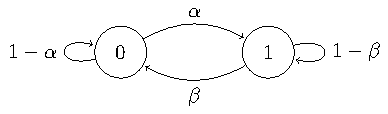
\includegraphics{math2750_files/figure-latex/twostate-1} 

}

\caption{Transition diagram for the two-state Markov chain}\label{fig:twostate}
\end{figure}

We can use this as a simple model of a broken printer, for example. If the printer is broken (state 0) on one day, then with probability \(\alpha\) it will be fixed (state 1) by the next day; while if it is working (state 1), then with probability \(\beta\) it will have broken down (state 0) by the next day.

\begin{example}
\protect\hypertarget{exm:printer}{}\label{exm:printer}

\emph{If the printer is working on Monday, what's the probability that it also is working on Wednesday?}

If we call Monday day \(n\), then Wednesday is day \(n+2\), and we want to find the two-step transition probability.
\[ p_{11}(2) = \mathbb P (X_{n+2} = 1 \mid X_n = 1) . \]
The key to calculating this is to \emph{condition on the first step} again -- that is, on whether the printer is working on Tuesday. We have
\begin{align*}
  p_{11}(2) &= \mathbb P (X_{n+1} = 0 \mid X_n = 1)\,\mathbb P (X_{n+2} = 1 \mid X_{n+1} = 0, X_n = 1) \\
  &\qquad{} + \mathbb P (X_{n+1} = 1 \mid X_n = 1)\,\mathbb P (X_{n+2} = 1 \mid X_{n+1} = 1, X_n = 1) \\
  &= \mathbb P (X_{n+1} = 0 \mid X_n = 1)\,\mathbb P (X_{n+2} = 1 \mid X_{n+1} = 0) \\
  &\qquad{} + \mathbb P (X_{n+1} = 1 \mid X_n = 1)\,\mathbb P (X_{n+2} = 1 \mid X_{n+1} = 1) \\
  &= p_{10}p_{01} + p_{11}p_{11} \\
  &= \beta\alpha + (1-\beta)^2 .
\end{align*}
In the second equality, we used the Markov property to mean conditional probabilities like \(\mathbb P(X_{n+2} = 1 \mid X_{n+1} = k)\) did not have to depend on \(X_n\).

Another way to think of this as we summing the probabilities of all length-2 paths from 1 to 1, which are \(1\to 0\to 1\) with probability \(\beta\alpha\) and \(1 \to 1 \to 1\) with probability \((1-\beta)^2\)

\end{example}

\hypertarget{n-step}{%
\subsection{\texorpdfstring{\emph{n}-step transition probabilities}{n-step transition probabilities}}\label{n-step}}

In the above example, we calculated a two-step transition probability \(p_{ij}(2) = \mathbb P (X_{n+2} = j \mid X_n = i)\) by conditioning on the first step. That is, by considering all the possible intermediate steps \(k\), we have
\[ p_{ij}(2) = \sum_{k\in\mathcal S} \mathbb P (X_{n+1} = k \mid X_n = i)\mathbb P (X_{n+2} = j \mid X_{n+1} = k) = \sum_{k\in\mathcal S} p_{ik}p_{kj} . \]

But this is exactly the formula for multiplying the matrix \(\mathsf P\) with itself! In other words, \(p_{ij}(2) = \sum_{k} p_{ik}p_{kj}\) is the \((i,j)\)th entry of the matrix square \(\mathsf P^2 = \mathsf{PP}\). If we write \(\mathsf P(2) = (p_{ij}(2))\) for the matrix of two-step transition probabilities, we have \(\mathsf P(2) = \mathsf P^2\).

More generally, we see that this rule holds over multiple steps, provided we sum over all the possible paths \(i\to k_1 \to k_2 \to \cdots \to k_{n-1} \to j\) of length \(n\) from \(i\) to \(j\).

\begin{theorem}
\protect\hypertarget{thm:thm-n-step}{}\label{thm:thm-n-step}

Let \((X_n)\) be a Markov chain with state space \(\mathcal S\) and transition matrix \(\mathsf P = (p_{ij})\). For \(i,j \in \mathcal S\), write
\[ p_{ij}(n) = \mathbb P(X_n = j \mid X_0 = i) \]
for the \(n\)-step transition probability. Then
\[ p_{ij}(n) = \sum_{k_1, k_2, \dots, k_{n-1} \in \mathcal S} p_{ik_1} p_{k_1k_2} \cdots p_{k_{n-2}k_{n-1}} p_{k_{n-1}j} . \]
In particular, \(p_{ij}(n)\) is the \((i,j)\)th element of the matrix power \(\mathsf P^n\), and the matrix of \(n\)-step transition probabilities is given by \(\mathsf P(n) = \mathsf P^n\).

\end{theorem}

The so-called \textbf{Chapman--Kolmogorov equations} follow immediately from this.

\begin{theorem}[Chapman–Kolmogorov equations]
\protect\hypertarget{thm:c-k}{}\label{thm:c-k}

Let \((X_n)\) be a Markov chain with state space \(\mathcal S\) and transition matrix \(\mathsf P = (p_{ij})\). Then, for non-negative integers \(n,m\), we have
\[ p_{ij}(n+m) = \sum_{k \in \mathcal S} p_{ik}(n)p_{kj}(m) , \]
or, in matrix notation, \(\mathsf P(n+m) = \mathsf P(n)\mathsf P(m)\).

\end{theorem}

In other words, a trip of length \(n + m\) from \(i\) to \(j\) is a trip of length \(n\) from \(i\) to some other state \(k\), then a trip of length \(m\) from \(k\) back to \(j\), and this intermediate stop \(k\) can be any state, so we have to sum the probabilities.

Of course, once we know that \(\mathsf P(n) = \mathsf P^n\) is given by the matrix power, it's clear to see that \(\mathsf P(n+m) = \mathsf P^{n+m} = \mathsf P^n \mathsf P^m = \mathsf P(n)\mathsf P(m)\).

\begin{example}
\protect\hypertarget{exm:printer2}{}\label{exm:printer2}

In our two-state broken printer example above, the matrix of two-state transition probabilities is given by
\begin{align*}
\mathsf P(2) = \mathsf P^2 &=  \begin{pmatrix} 1-\alpha & \alpha \\ \beta & 1-\beta \end{pmatrix}  \begin{pmatrix} 1-\alpha & \alpha \\ \beta & 1-\beta \end{pmatrix} \\
&=  \begin{pmatrix} (1-\alpha)^2 + \alpha\beta & (1-\alpha)\alpha + \alpha(1-\beta) \\ \beta(1-\alpha) + (1-\beta)\beta & \beta\alpha + (1-\beta)^2 \end{pmatrix} ,
\end{align*}
where the bottom right entry \(p_{11}(2)\) is what we calculated earlier.

\end{example}

One final comment. It's also convenient to consider the initial distribution \(\boldsymbol\lambda = (\lambda_i)\) as a \emph{row} vector. The first-step distribution is given by
\[ \mathbb P(X_1 = j) = \sum_{i \in \mathcal S} \lambda_i p_{ij} , \]
by conditioning on the start point.
This is exactly the \(j\)th element of the vector--matrix multiplication \(\boldsymbol\lambda \mathsf P\). More generally, the row vector of of probabilities after \(n\) steps is given by \(\boldsymbol\lambda \mathsf P^n\).

In the next section, we look at how to model some actuarial problems using Markov chains.

\hypertarget{S06-examples}{%
\section{Examples from actuarial science}\label{S06-examples}}

\begin{itemize}
\tightlist
\item
  Three Markov chain models for insurance problems
\end{itemize}

In this lecture we'll set up three simple models for an insurance company that can be analysed using ideas about Markov chains. The first example has a direct Markov chain model. For the second and third examples, we will have to be clever to find a Markov chain associated to the situation.

\hypertarget{S06-example1}{%
\subsection{A simple no-claims discount model}\label{S06-example1}}

A motor insurance company puts policy holders into three categories:

\begin{itemize}
\tightlist
\item
  no discount on premiums (state 1)
\item
  25\% discount on premiums (state 2)
\item
  50\% discount on premiums (state 3)
\end{itemize}

New policy holders start with no discount (state 1). Following a year with no insurance claims, policy holders move up one level of discount. If they start the year in state 3 and make no claim, they remain in state 3. Following a year with at least one claim, they move down one level of discount. If they start the year in state 1 and make at least one claim, they remain in state 1. The insurance company believes that probability that a motorist has a claim free year is \(\frac34\).

We can model this directly as a Markov chain:

\begin{itemize}
\tightlist
\item
  the state space \(\mathcal S = \{1,2,3\}\) is discrete;
\item
  the time index is discrete, as we have one discount level each year;
\item
  the probability of being in a certain state at a future time is completely determined by the present state (the Markov property);
\item
  the one-step transition probabilities are not time dependent (time homogeneous).
\end{itemize}

The transition probability and transition diagram of the Markov chain are:
\[ \mathsf P = \begin{pmatrix} \frac14 & \frac34 & 0 \\ \frac14 & 0 & \frac34 \\ 0 & \frac14 & \frac34 \end{pmatrix} . \]

\begin{figure}

{\centering 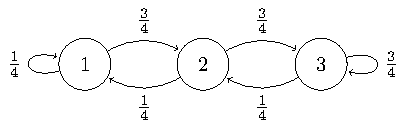
\includegraphics{math2750_files/figure-latex/example1-1} 

}

\caption{Transition diagram for the simple no-claims discount model}\label{fig:example1}
\end{figure}

\begin{example}
\protect\hypertarget{exm:act1}{}\label{exm:act1}

\emph{What is the probability of having a 50\% reduction to your premium three years from now, given that you currently have no reduction on the premium?}

We want to find the three-step transition probability
\[
p_{13}(3) = \mathbb P(X_{3} = 3 \mid X_0=1) .
\]
We can find this by summing over all paths \(1 \to k_1 \to k_2 \to 3\). There are two such paths, \(1 \to 1 \to 2 \to 3\) and \(1 \to 2 \to 3 \to 3\). Thus
\[ p_{13}(3) = p_{11}p_{12}p_{23} + p_{12}p_{23}p_{33} = \frac14 \cdot\frac34 \cdot\frac34 + \frac34 \cdot\frac34 \cdot\frac34 = \frac{36}{64} = \frac{9}{16} . \]

Alternatively, we could directly calculate all the three-step transition probabilities by the matrix method, to get
\[ \mathsf P(3) = \mathsf P^3 = \mathsf{PPP} = \frac{1}{64} \begin{pmatrix} 7 & 21 & 36 \\ 7 & 12 & 45 \\ 4 & 15 & 45 \end{pmatrix} .\]
(You can check this yourself, if you want.) The desired \(p_{13}(3)\) is the top right entry \(36/64 = 9/16\).

\end{example}

\hypertarget{S06-example2}{%
\subsection{An accident model with memory}\label{S06-example2}}

Sometimes, we are presented with a situation where the ``obvious'' stochastic process is not a Markov chain. But sometimes we can find a related process that \emph{is} a Markov chain, and study that instead. As an example of this, we consider at a different accident model.

According to a different model, a motorist's \(n\)th year of driving is either accident free, or has exactly one accident. (The model does not allow for more than one accident in a year.) Let \(Y_n\) be a random variable so that,
\[
Y_n=\begin{cases}
0&\text{ if the motorist has no accident in year $n$,}\\
1&\text{ if the motorist has one accident in year $n$.}
\end{cases}
\]
This defines a stochastic process \((Y_n)\) with finite state space \(\mathcal{S}=\{0,1\}\) and discrete time \(n = 1,2,3,\dots\).

The probability of an accident in year \(n+1\) is modelled as a function of the total number of previous accidents over a function of the number of years in the policy; that is,
\[
\mathbb P(Y_{n+1}= 1 \mid Y_n=y_{n},\dots ,Y_2=y_{2},Y_1=y_{1} )=\frac{f(y_1+y_2+\cdots +y_n)}{g(n)},
\]
and \(Y_{n+1} = 0\) otherwise,
where \(f\) and \(g\) are non-negative increasing functions with \(0\leq f(m)\leq g(m)\) for all \(m\). (We'll come back to these conditions in a moment.)

Unfortunately \((Y_n)\) is \emph{not} a Markov chain -- it's clear that \(Y_{n+1}\) depends not only on \(Y_n\), the number accidents this year, but the entire history \(Y_1, Y_2, \dots, Y_n\).

However, we have a cunning work-around. Define \(X_n=\sum_{i=1}^n Y_i\) to be the total number of accidents up to year \(n\). Then \((X_n)\) \emph{is} a Markov chain. In fact, we have
\begin{align*}
    \mathbb P(X_{n+1}={}&{}x_{n}+1\mid X_n=x_n, \dots, X_2=x_2, X_1=x_1)\\
    &=\mathbb P(Y_{n+1}=1\mid Y_n=x_n - x_{n-1}, \dots Y_2=x_2-x_1, Y_1=x_1)\\
    &=\frac{f\big((x_n-x_{n-1}) +\cdots +(x_2-x_1) + x_1\big)}{g(n)}\\
    &=\frac{f(x_n)}{g(n)},
\end{align*}
and \(X_{n+1} = x_n\) otherwise. This clearly depends only on \(x_n\). Thus we can use Markov chain techniques on \((X_n)\) to lean about the non-Markov process \((Y_n)\).

Note that the probability that \(X_{n+1} = x_n\) or \(x_n+ 1\) depends not only on \(x_n\) but also on the time \(n\). So this is a rare example of a time \emph{inhomogeneous} Markov process, where the transition probabilities do depend on the time \(n\).

Before we move on, let's think about the conditions we placed on this model. First, the condition that \(f\) is increasing means that between drivers who have been driving the same number of years, we think the more accident-prone in the past is more likely to have an accident in the future. Second, the condition that \(g\) is increasing means that between drivers who have had the same number of accidents, we think the one who has spread those accidents over a longer period of time is less likely to have accidents in the future. Third, the transition probabilities should lie in the range \([0,1]\); but since \(\sum_{i=1}^m y_i\leq m\), our condition \(0\leq f(m)\leq g(m)\) guaranteed that this is the case.

\hypertarget{S06-example3}{%
\subsection{A no-claims discount model with memory}\label{S06-example3}}

Sometimes, we are presented with a stochastic process which is not a Markov chain, but where by altering the state space \(\mathcal{S}\) we \emph{can} end up with a process which \emph{is} a Markov chain. As such, when making a model, it is important to think carefully about choice of state space. To see this we will return to the no-claims discount example.

Suppose now we have an model with four levels of discount:

\begin{itemize}
\tightlist
\item
  no discount (state 1)
\item
  20\% discount (state 2)
\item
  40\% discount (state 3)
\item
  60\% discount (state 4)
\end{itemize}

If a year is accident free, then the discount increases one level, to a maximum of 60\%. This time, if the year has an accident, then the discount decreases by one level if the year previous to that was accident free, but decreases by \emph{two} levels if the previous year had an accident as well, both to a minimum of no discount.

As before, the insurance company believes that probability that a motorist has a claim-free year is \(\frac34 = 0.75\).

We might consider the most natural choice of a state space, where the states are discount levels; say, \(\mathcal{S}=\{1,2,3,4\}\). But this is not a Markov chain, since if a policy holder has an accident, we may need to know about the past in order to determine probabilities for future states, which violates the Markov property. In particular, if a motorist is in state 3 (40\% discount) and has an accident, they will either move down to level 2 (if they had not crashed the previous year, so had previously been in state 2) or to level 1 (if they had crashed the previous year, so had previously been in state 4) -- but that depends on their previous level too, which the Markov property doesn't allow. (You can check this is the only violation of the Markov property.)

However, we can be clever again, this time in the choice of our state space. Instead, we can split the 40\% level into two different states: state ``3a'' if there was no accident the previous year, and state ``3b'' if there was an accident the previous year. Our states are now:

\begin{itemize}
\tightlist
\item
  no discount (state 1)
\item
  20\% discount (state 2)
\item
  40\% discount, no claim in previous year (state 3a)
\item
  40\% discount, claim in previous year (state 3b)
\item
  60\% discount (state 4)
\end{itemize}

Now this \emph{is} a Markov chain, because the new states 3s carry with them the memory of the previous year, to ensure the Markov property is preserved. Under the assumption of 25\% of drivers having an accident each year, the transition matrix is
\[
\mathsf P=\begin{pmatrix}
0.25 & 0.75 & 0 & 0 & 0\\
0.25 & 0 & 0.75 & 0 & 0\\
0 & 0.25 & 0 & 0 & 0.75\\
0.25 & 0 & 0 & 0 & 0.75\\
0 & 0 & 0 & 0.25 & 0.75\end{pmatrix}.
\]
The transition diagram is shown below. (Recall that we don't draw arrows with probability 0.)

\begin{figure}

{\centering 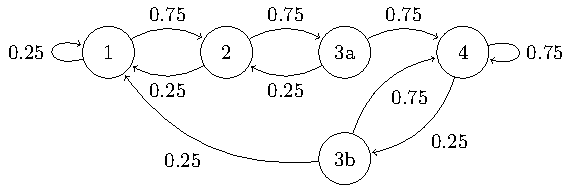
\includegraphics{math2750_files/figure-latex/example3-1} 

}

\caption{Transition diagram for the no-claims discount model with memory}\label{fig:example3}
\end{figure}

Note that when we move up from state 2, we go to 3a (no accident in the previous year); but when we move down from state 4, we go to 3b (accident in the previous year).

\textbf{In the next section}, we look at how to study big Markov chains by splitting them into smaller pieces called ``classes''.

\hypertarget{P03}{%
\section*{Problem sheet 3}\label{P03}}
\addcontentsline{toc}{section}{Problem sheet 3}

\commfalse

You should attempt all these questions and write up your solutions in advance of your workshop in week 4 (Monday 15 or Tuesday 16 February) where the answers will be discussed.

\textbf{1.} Consider a Markov chain with state space \(\mathcal S = \{1,2,3\}\), and transition matrix partially given by
\[ \mathsf P = \begin{pmatrix} ? & 0.3 & 0.3 \\ 0.2 & 0.4 & ? \\ ? & ? & 1 \end{pmatrix} . \]

\textbf{(a)} Replace the four question marks by the appropriate transition probabilities.

\begin{myanswers}

\emph{Solution.} Rows must add up to 1 and every entry must be non-negative, so the transition matrix is
\[ \mathsf P = \begin{pmatrix} 0.4 & 0.3 & 0.3 \\ 0.2 & 0.4 & 0.4 \\ 0 & 0 & 1 \end{pmatrix} . \]

\end{myanswers}

\textbf{(b)} Draw a transition diagram for this Markov chain.

\begin{myanswers}

\emph{Solution.}

\begin{figure}

{\centering 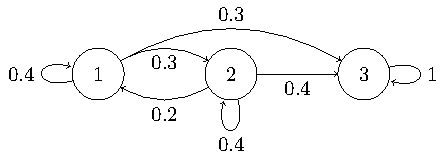
\includegraphics{math2750_files/figure-latex/Q31-1} 

}

\caption{Transition diagram for Question 1.}\label{fig:Q31}
\end{figure}

\end{myanswers}

\textbf{(c)} Find the matrix \(\mathsf P(2)\) of two-step transition probabilities.

\begin{myanswers}

\emph{Solution.} \({\displaystyle \mathsf P(2) = \mathsf P^2 = \begin{pmatrix} 0.22 & 0.24 & 0.54 \\ 0.16 & 0.22 & 0.62 \\ 0 & 0 & 1 \end{pmatrix}}\)

\end{myanswers}

\textbf{(d)} By summing the probabilities of all relevant paths, find the three-step transition probability \(p_{13}(3)\).

\begin{myanswers}

\emph{Solution.} There are seven relevant paths: \(1 \to 1 \to 1 \to 3\), \(1 \to 1 \to 2 \to 3\), \(1 \to 1 \to 3 \to 3\), \(1 \to 2 \to 1 \to 3\), \(1 \to 2 \to 2 \to 3\), \(1 \to 2 \to 3 \to 3\), and \(1 \to 3 \to 3 \to 3\). So
\begin{align*}
p_{13}(3) &= p_{11}p_{11}p_{11}p_{13} + p_{11}p_{12}p_{23} + p_{11}p_{13}p_{33}  + p_{12} p_{21} p_{13}\\
& \qquad{}+ p_{12}p_{22}p_{23} + p_{12}p_{23}p_{33} + p_{13}p_{33}p_{33}\\
& = 0.4 \cdot 0.4 \cdot 0.3 + 0.4\cdot 0.3\cdot 0.4 + 0.4\cdot 0.3 \cdot 1 + 0.3 \cdot 0.2 \cdot 0.3 \\
& \qquad{}+ 0.3\cdot 0.4 \cdot 0.4 + 0.3 \cdot 0.4 \cdot 1 + 0.3 \cdot 1 \cdot 1\\
&= 0.702
\end{align*}

\end{myanswers}

\textbf{2.} Consider a Markov chain \((X_n)\) which moves between the vertices of
a tetrahedron.

At each time step, the process randomly chooses one of the edges connected to the current vertex and follows it to a new vertex. The edge to follow is selected randomly with all options having equal probability and each selection is independent of the past movements. Let \(X_n\) be the vertex the process is in after step \(n\).

\textbf{(a)} Write down the transition matrix \(\mathsf P\) of this Markov chain.

\begin{myanswers}

The chain can move from a state to any of the other \(3\) states, each with probability \(1/3\). So
\[ \mathsf P = \begin{pmatrix} 0 & \frac13 & \frac13 & \frac13 \\
                               \frac13 & 0 & \frac13 & \frac13 \\
                               \frac13 & \frac13 & 0 & \frac13 \\
                               \frac13 & \frac13 & \frac13 & 0 \end{pmatrix} . \]

\end{myanswers}

\textbf{(b)} By summing over all relevant paths of length two, calculate the two-step transition probabilities \(p_{11}(2)\) and \(p_{12}(2)\). Hence, write down the two-step transition matrix \(\mathsf P(2)\).

\begin{myanswers}

The length-2 paths from 1 to 1 are \(1 \to k \to 1\) for \(k = 2,3,4\), so
\[ p_{11}(2) = p_{12}p_{21} + p_{13}p_{31} + p_{14}p_{41} = \tfrac13 \tfrac13 +  \tfrac13 \tfrac13 + \tfrac13 \tfrac13 = \tfrac13  .   \]
The length-2 paths from 1 to 2 are \(1 \to 3 \to 2\) and \(1 \to 4 \to 2\), so
\[ p_{12}(2) = p_{13}p_{32} + p_{14}p_{42} = \tfrac13 \tfrac13 + \tfrac13 \tfrac13 = \tfrac29 . \]

By symmetry, \(p_{ii}(2) = p_{11}(2)\) for all \(i\), and \(p_{ij}(2) = p_{12}(2)\) for all \(i \neq j\). Therefore
\[ \mathsf P(2) = \begin{pmatrix} \frac13 & \frac29 & \frac29 & \frac29 \\
                               \frac29 & \frac13 & \frac29 & \frac29 \\
                               \frac29 & \frac29 & \frac13 & \frac29 \\
                               \frac29 & \frac29 & \frac29 & \frac13 \end{pmatrix} . \]

\end{myanswers}

\textbf{(c)} Check your answer by calculating the matrix square \(\mathsf P^2\).

\begin{myanswers}

We can verify that
\[ \mathsf P^2 = \begin{pmatrix} 0 & \frac13 & \frac13 & \frac13 \\
\frac13 & 0 & \frac13 & \frac13 \\
\frac13 & \frac13 & 0 & \frac13 \\
\frac13 & \frac13 & \frac13 & 0 \end{pmatrix} \begin{pmatrix} 0 & \frac13 & \frac13 & \frac13 \\
\frac13 & 0 & \frac13 & \frac13 \\
\frac13 & \frac13 & 0 & \frac13 \\
\frac13 & \frac13 & \frac13 & 0 \end{pmatrix}=
\begin{pmatrix} \frac13 & \frac29 & \frac29 & \frac29 \\
\frac29 & \frac13 & \frac29 & \frac29 \\
\frac29 & \frac29 & \frac13 & \frac29 \\
\frac29 & \frac29 & \frac29 & \frac13 \end{pmatrix} , \]
as above.

\end{myanswers}

\begin{figure}

{\centering 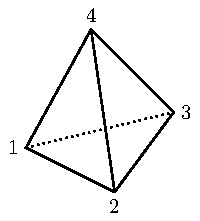
\includegraphics[width=850em]{math2750_files/figure-latex/testing-1} 

}

\caption{A tetrahedron}\label{fig:testing}
\end{figure}

\textbf{3.} Consider the two-state ``broken printer'' Markov chain, with state space \(\mathcal S = \{0,1\}\), transition matrix
\[ \mathsf P = \begin{pmatrix} 1-\alpha & \alpha \\
                 \beta & 1-\beta \end{pmatrix} \]
with \(0 < \alpha, \beta < 1\), and initial distribution \(\boldsymbol\lambda = (\lambda_0, \lambda_1)\). Write \(\mu_n =\mathbb P(X_n = 0)\).

\textbf{(a)} By writing \(\mu_{n+1}\) in terms of \(\mu_n\), show that we have
\[ \mu_{n+1} - \big(1-(\alpha+\beta)\big)\mu_n = \beta . \]

\begin{myanswers}

Using the law of total probability, we have
\begin{multline*}
\mathbb P(X_{n+1} = 0) = \mathbb P(X_n = 0)\,\mathbb P(X_{n+1} = 0 \mid X_n = 0) \\
+ \mathbb P(X_n = 1)\,\mathbb P(X_{n+1} = 0 \mid X_n = 1) ,
\end{multline*}
which in terms of \((\mu_n)\) is
\[ \mu_{n+1} = \mu_n (1-\alpha) + (1 - \mu_n)\beta . \]
We used here that \(\mathbb P(X_n = 1) = 1-\mu_n\).
Rearranging this gives the answer.

\end{myanswers}

\textbf{(b)} By solving this linear difference equation using the initial condition \(\mu_0 = \lambda_0\), or otherwise, show that
\[ \mu_n = \frac{\beta}{\alpha+\beta} + \left(\lambda_0 - \frac{\beta}{\alpha+\beta}\right)\big(1-(\alpha+\beta)\big)^n   . \]

\begin{myanswers}

The characteristic equation is \(\lambda - (1-(\alpha+\beta)) = 0\) with a single root at \(\lambda = 1 - (\alpha+\beta)\). The general solution to the homogeneous equation is, therefore, \(A(1-(\alpha+\beta))^n\).

For a particular solution, we guess a solution \(\mu_n = C\), and \(C - (1-(\alpha+\beta))C = \beta\) gives \(C = \beta/(\alpha+\beta)\). Thus the general solution to the inhomogeneous equation is
\[ \mu_n = \frac{\beta}{\alpha+\beta} + A\big(1-(\alpha+\beta)\big)^n .\]

From the initial condition, we get \(\lambda_0 = \beta/(\alpha+\beta) + A\), and therefore \(A = \lambda_0 - \beta/(\alpha+\beta)\). The solution is therefore as given.

\end{myanswers}

\textbf{(c)} What, therefore, are \(\lim_{n\to\infty} \mathbb P(X_n = 0)\) and \(\lim_{n\to\infty} \mathbb P(X_n = 1)\)?

\begin{myanswers}

Note that \(-1 < 1 - (\alpha + \beta) < 1\), so \((1-(\alpha+\beta))^n \to 0\). Therefore we have
\begin{align*}
\lim_{n\to\infty} \mathbb P(X_n = 0) &= \lim_{n\to\infty} \mu_n \\
&= \lim_{n\to\infty} \left( \frac{\beta}{\alpha+\beta} + \left(\lambda_0 - \frac{\beta}{\alpha+\beta}\right)\big(1-(\alpha+\beta)\big)^n \right) \\
&= \frac{\beta}{\alpha+\beta} .
\end{align*}
Since \(\mathbb P(X_n = 1) = 1- \mathbb P(X_n = 0)\), we have
\[ \mathbb P(X_n = 1) \to 1 - \frac{\beta}{\alpha+\beta} = \frac{\alpha}{\alpha+\beta} . \]

\end{myanswers}

\textbf{(d)} Explain what happens if the Markov chain is started in the distribution
\[ \lambda_0 = \frac{\beta}{\alpha+\beta} , \qquad \lambda_1 = \frac{\alpha}{\alpha+\beta}  . \]

\begin{myanswers}

Substituting in the value of \(\lambda_0\) into the equation for \(\mu_n\), the second term cancel, and we have that \(\mathbb P(X_n = 0) = \mu_n = \beta/(\alpha+\beta)\) for all times \(n\), and therefor \(\mathbb P(X_n = 1) = \alpha/(\alpha+\beta)\) too. This means that the Markov chain remains in the same ``stationary distribution'' forever.

\end{myanswers}

\textbf{4.} Let \((X_n)\) be a Markov chain. Show that, for any \(m \geq 1\), we have
\[ \mathbb P(X_{n+m} = x_{n+m} \mid X_n = x_n, X_{n-1} = x_{n-1}, \dots, X_0 = x_0)  =  \mathbb P(X_{n+m} = x_{n+m} \mid X_n = x_n) . \]

\begin{myanswers}

Note that we have a sequence of statements here, for \(m = 1, 2, \dots\). Note also that the case \(m = 1\) is the standard Markov property. When we have a sequence of statements and we can easily prove the first one, this is a good sign that a proof by induction is the way to go.

Before starting, for reasons of space, we adopt notation where we suppress the capital \(X\)s, so we want to show that
\[ \mathbb P(x_{n+m} \mid x_n, x_{n-1}, \dots, x_0 ) = \mathbb P(x_{n+m} \mid x_n) . \]

We work by induction on \(m\). The base case \(m = 1\) is the standard Markov property.

Assume the inductive hypothesis: that result holds for \(m\). We now need to prove the inductive step: that the result holds for \(m+1\). For \(m+1\) we have, by conditioning on the first step \(x_{n+1}\),
\begin{multline*} \mathbb P(x_{n+m+1} \mid x_n, x_{n-1}, \dots, x_0 ) \\
 = \sum_{x_{n+1}} \mathbb P(x_{n+1} \mid x_n, x_{n-1}, \dots, x_0 )\,\mathbb P(x_{n+m+1} \mid x_{n+1}, x_n, x_{n-1}, \dots, x_0 )     \end{multline*}
By the standard Markov property the first term simplifies to \(\mathbb P(x_{n+1} \mid x_n)\), and by the result for \(m\) the second term simplifies to \(\mathbb P(x_{n+m+1} \mid x_{n+1})\). So we have
\[ \mathbb P(x_{n+m+1} \mid x_n, x_{n-1}, \dots, x_0 ) = \sum_{x_{n+1}} \mathbb P(x_{n+1} \mid x_n) \mathbb P(x_{n+m+1} \mid x_{n+1}) . \]
But the right-hand side here is \(\mathbb P(x_{n+m+1} \mid x_n)\) written using conditioning on the first step and using the result for \(m\). By induction, we are done.

\end{myanswers}

\textbf{5.} A car insurance company operates a no-claims discount system for existing policy holders. The possible discounts on premiums are \(\{0\%,25\%,40\%,50\%\}\). Following a claim-free year, a policyholder's discount level increases by one level (or remains at 50\% discount). If the policyholder makes one or more claims in a year, the discount level decreases by one level (or remains at 0\% discount).

The insurer believes that the probability of of making at least one claim in a year is \(0.1\) if the previous year was claim-free and \(0.25\) if the previous year was not claim-free.

\textbf{(a)} Explain why we cannot use \(\{0\%,25\%,40\%,50\%\}\) as the state space of a Markov chain to model discount levels for policyholders.

\begin{myanswers}

The Markov property does not hold for the time-homogeneous process described since the probability of moving to a given state at the next time step is not simply dependent on the current state if \(\mathcal S=\{0\%,25\%,40\%,50\%\}\). For example,
\[
    \mathbb P(X_{n+1}=25\% \mid X_n= 40\% )=\begin{cases} 
    0.25 & \text{if $X_{n-1}=50\%$}\\
    0.1 & \text{if $X_{n-1}=25\%$.} \end{cases} \]

\end{myanswers}

\textbf{(b)} By considering additional states, show that a Markov chain can be used to model the discount level.

\begin{myanswers}

The problem is that the process has a memory of the previous year.
If we currently have a discount of 0\%, we know a claim was made in the year before, so no changes are required. Similarly, at 50\% discount, we know that no claim was made in the previous year. The other two states, 25\% and 40\%, have different behaviour depending on whether or not there was a claim in the previous year.

So we will split each of these into two states: 25+ will denote a 25\% discount with no claim in the previous year, while 25- will denote a 25\% discount with a claim in the previous year. We define the state 40+ and 40- similarly. Then we have a Markov chain, since the current state and the number of claims in the previous year completely defines the distribution on future behaviour.

\end{myanswers}

\textbf{(c)} Draw the transition diagram and write down the transition matrix.

\begin{myanswers}

The transition diagram is as shown below.

\begin{figure}

{\centering 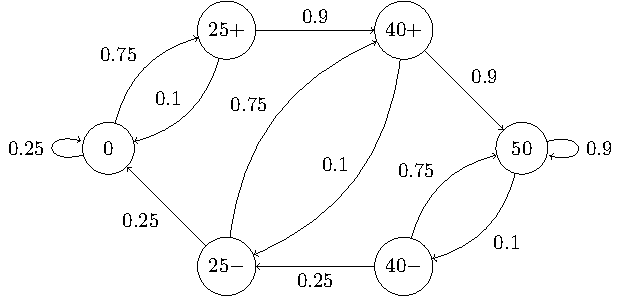
\includegraphics{math2750_files/figure-latex/fortyplus-1} 

}

\caption{Transition diagram for the car insurance Markov chain}\label{fig:fortyplus}
\end{figure}

The transition matrix is given by,
\[ \mathsf P = 
    \begin{matrix}
    & \begin{matrix} 
        0 & 25+ & 25- & 40+ & 40- & 50
      \end{matrix} \\
    \begin{matrix}
      0 \\ 25+ \\ 25- \\ 40+ \\ 40- \\ 50
    \end{matrix}
    &
    \begin{pmatrix}
    0.25 & 0.75 & 0    & 0    & 0   & 0    \\
      0.1  & 0    & 0    & 0.9  & 0   & 0    \\
      0.25 & 0    & 0    & 0.75 & 0   & 0    \\
      0    & 0    & 0.1  & 0    & 0   & 0.9  \\
      0    & 0    & 0.25 & 0    & 0   & 0.75 \\
      0    & 0    & 0    & 0    & 0.1 & 0.9 
    \end{pmatrix}
    \end{matrix}
    \]

\end{myanswers}

\textbf{6.} The credit rating of a company can be modelled as a Markov chain. Assume the rating is assessed once per year at the end of the year and possible ratings are A (good), B (fair) and D (in default). The transition matrix is
\[\mathsf P=\begin{pmatrix} 0.92&0.05&0.03\\
0.05&0.85&0.1\\
0&0&1 \end{pmatrix} . \]

\textbf{(a)} Calculate the two-step transition probabilities, and hence find the expected number of defaults in the next two years from \(100\) companies all rated A at the start of the period.

\begin{myanswers}

The matrix of two-step transition probabilities is given by the matrix square
\[\mathsf P(2) = \mathsf P^2= \begin{pmatrix} 0.8489&0.0885&0.0626\\
0.0885&0.7250&0.1865\\
0&0&1 \end{pmatrix}. \]
The number of defaults in two years from \(100\) A-rated companies is \(100 \times p_{\mathrm{AD}}(2) = 100 \times 0.0626 = 6.26\).

\end{myanswers}

\textbf{(b)} What is the probability that a company rated A will at some point default without ever having been rated B in the meantime?

\begin{myanswers}

Let \(\delta\) be the desired probability that an A-rated company will default without having been rated B. We condition on the first step: with probability \(0.92\) we remain in state A, and by the Markov property the probability of the given event remains at \(\delta\); with probability \(0.05\) we move to state B, and the event fails to occur; and with probability \(0.03\) we move to state D and the event occurs immediately. Therefore, we have
\[ \delta = 0.92\delta + 0.05\times 0 + 0.03 \times 1 = 0.92\delta + 0.03 ,  \]
which has solution \(\delta = 0.03/(1-0.92) = 0.375\).

\end{myanswers}

A corporate bond portfolio manager follows an investment strategy which means that bonds which falls from A-rated to B-rated is sold and replaced with an A-rated bond. The manger believes this will improve the returns on the portfolio because it will reduce the number of defaults experienced.

\textbf{(c)} Calculate the expected number of defaults in the manager's portfolio over the next two years given there are initially 100 A-rated bonds.

\begin{myanswers}

Given that B-rated bonds are replaced by A-rated bonds, we have a new Markov chain with state space \(\{\mathrm{A},\mathrm{D}\}\) and transition matrix
\[ \mathsf P = \begin{pmatrix} 0.92+0.05 & 0.03 \\ 0 & 1 \end{pmatrix} =  \begin{pmatrix} 0.97 & 0.03 \\ 0 & 1 \end{pmatrix} .  \]
The two-step transition probability is
\[ \mathsf P(2) = \mathsf P^2 =  \begin{pmatrix} 0.97 & 0.03 \\ 0 & 1 \end{pmatrix} \begin{pmatrix} 0.97 & 0.03 \\ 0 & 1 \end{pmatrix} = \begin{pmatrix} 0.9409 & 0.0591 \\ 0 & 1 \end{pmatrix} .  \]
Thus the number of defaults from \(100\) A-rated bonds in two years is \(100\times p_{\mathrm{AD}}(2) = 100\times 0.0591 = 5.91\). The manager was right: this is slightly less than the \(6.26\) from part (a).

\end{myanswers}

\hypertarget{S07-classes}{%
\section{Class structure}\label{S07-classes}}

\begin{itemize}
\tightlist
\item
  Communicating classes and irreducibility
\item
  Period of a state (and class)
\end{itemize}

\hypertarget{comm-classes}{%
\subsection{Communicating classes}\label{comm-classes}}

If we have a large complicated Markov chain, it can be useful to split the state space up into smaller pieces that can be studied separately. The idea is that states \(i\) and \(j\) should definitely be in the same piece (or "class) if we can get from \(i\) to \(j\) and then back to \(i\) again after some number of steps.

\begin{definition}
\protect\hypertarget{def:comm}{}\label{def:comm}

Consider a Markov chain on a state space \(\mathcal S\) with transition matrix \(\mathsf P\). We say that state \(j\in\mathcal{S}\) is \textbf{accessible} from state \(i\in\mathcal{S}\) and write \(i \to j\) if, for some \(n\), \(p_{ij}(n)>0\).

If \(i \to j\) and \(j \to i\), we say that \(i\) \textbf{communicates with} \(j\) and write \(i \leftrightarrow j\).

\end{definition}

Here, the condition \(p_{ij}(n)>0\) means that, starting from \(i\), there's a positive chance that we'll get to \(j\) at some point in the future -- hence the term ``accessible''.

\begin{theorem}
\protect\hypertarget{thm:equiv-rel}{}\label{thm:equiv-rel}

Consider a Markov chain on a state space \(\mathcal S\) with transition matrix \(\mathsf P\). Then the ``communicates with'' relation \(\leftrightarrow\) is an \href{https://en.wikipedia.org/wiki/Equivalence_relation}{\textbf{equivalence relation}}; that is, it has the following properties:

\begin{itemize}
\tightlist
\item
  \textbf{reflexive}: \(i \leftrightarrow i\) for all \(i\);
\item
  \textbf{symmetric}: if \(i \leftrightarrow j\) then \(j \leftrightarrow i\);
\item
  \textbf{transitive}: if \(i \leftrightarrow j\) and \(j \leftrightarrow k\) then \(i \leftrightarrow k\).
\end{itemize}

\end{theorem}

\begin{proof}

\emph{Reflexivity}: Clearly \(p_{ii}(0) = 1 > 0\), because in ``zero steps'' we stay where we are. So \(i \leftrightarrow i\) for all \(i\).

\emph{Symmetry}: The definition of \(i \leftrightarrow j\) is symmetric under swapping \(i\) and \(j\).

\emph{Transitivity}. If we can get from \(i\) to \(j\) and we can get from \(j\) to \(k\), then we can get from \(i\) to \(k\) by going via \(j\). We just need to write that out formally.

Since \(i \to j\), we have \(p_{ij}(n) > 0\) for some \(n\), and since \(j \to k\), we also have \(p_{jk}(m) > 0\) for some \(m\). Then, by the Chapman--Kolmogorov equations, we have
\[ p_{ik}(n+m) = \sum_{l \in \mathcal S} p_{il}(n) p_{lk}(m) \geq p_{ij}(n) p_{jk}(m) > 0 , \]
from just picking out the \(l=j\) term in the sum. So \(i \to k\) too.

The same argument with \(k\) and \(i\) swapped gives \(k \to i\) also, so \(i \leftrightarrow k\).

\end{proof}

A fact you may remember about equivalence relations is that an equivalence relation, like \(\leftrightarrow\), partitions the space \(\mathcal S\) into \href{https://en.wikipedia.org/wiki/Equivalence_class}{\textbf{equivalence classes}}. This means that each state \(i\) is in exactly one equivalence class, and that class is the set of states \(j\) such that \(i \leftrightarrow j\). In this context, we call these \textbf{communicating classes}.

\begin{example}
\protect\hypertarget{exm:rw-class}{}\label{exm:rw-class}

In the simple random walk, provided \(p\) is not 0 or 1, every state communicates with every other state, because from \(i\) when can get to \(j > i\) by going up \(j - i\) times, and we can get to \(j < i\) by going down \(i - j\) times. Therefore the whole state space \(\mathcal S = \mathbb Z\) is one communicating class.

\end{example}

\begin{example}
\protect\hypertarget{exm:gamblers-class}{}\label{exm:gamblers-class}

Consider the gambler's ruin Markov chain on \(\{0,1,\dots,m\}\). There are three communicating classes. The ruin states \(\{0\}\) and \(\{m\}\) each don't communicate with any other states, so each are a class by themselves. The remaining states \(\{1,2,\dots,m-1\}\) are all in the same class, like the simple random walk.

\end{example}

\begin{example}
\protect\hypertarget{exm:hsd-class}{}\label{exm:hsd-class}

Consider the following simple model for an epidemic. We have three states: healthy (H), sick (S), and dead (D). This transition matrix is
\[ \mathsf P = \begin{pmatrix} p_{\mathrm{HH}} & p_{\mathrm{HS}} & 0 \\
p_{\mathrm{SH}} & p_{\mathrm{SS}} & p_{\mathrm{SD}} \\ 0 & 0 & 1 \end{pmatrix} ,    \]
and the transition diagram is:

\begin{figure}

{\centering 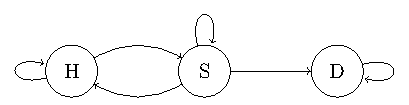
\includegraphics{math2750_files/figure-latex/HSD-1} 

}

\caption{Transition for the healthy--sick--dead chain.}\label{fig:HSD}
\end{figure}

Clearly H and S communicate with each other (you can become infected or recover), while D only communicates with itself (the dead do not recover). Hence, the state space \(\mathcal S = \{\mathrm{H},\mathrm{S},\mathrm{D}\}\) partitions into two communicating classes: \(\{\mathrm{H},\mathrm{S}\}\) and \(\{\mathrm{D}\}\).

\end{example}

A few more definitions that will be important later.

\begin{definition}
\protect\hypertarget{def:irreducible}{}\label{def:irreducible}

If the entire state space \(\mathcal S\) is one communicating class, we say that the Markov chain is \textbf{irreducible}.

We say that a communicating class is \textbf{closed} if no state outside the class is accessible from any state within the class. That is, class \(C \subset \mathcal S\) is closed if whenever there exist \(i \in C\) and \(j \in \mathcal S\) with \(i \to j\), then \(j \in C\) also. If a class is not closed, we say it is \textbf{open}.

If a state \(i\) is in a communicating class \(\{i\}\) by itself and that class is closed, then we say state \(i\) is \textbf{absorbing}.

\end{definition}

In non-maths language:

\begin{itemize}
\tightlist
\item
  An irreducible Markov chain can't be broken down into smaller pieces.
\item
  Once you enter a closed class, you can't leave that class.
\item
  Once you reach an absorbing state, you can't leave that state.
\end{itemize}

How do these work for our earlier examples?

\begin{example}
\protect\hypertarget{exm:ex-irred}{}\label{exm:ex-irred}

Going back to the previous examples:

\begin{itemize}
\tightlist
\item
  In the simple random walk, the whole state space is one communicating class which must therefore be closed. The Markov chain has only one class, so is irreducible.
\item
  In the gambler's ruin, classes \(\{0\}\) and \(\{m\}\) are closed, because the Markov chain stays there forever, and because these closed classes consist of only one state each, \(0\) and \(m\) are absorbing states. The class \(\{1, 2, \dots, m-1\}\) is open, as we can escape the class by going to \(0\) or \(m\). The gambler's ruin chain has multiple classes, so is not irreducible.
\item
  In the ``healthy--sick--dead'' chain, the class \(\{D\}\) is closed, so D is an absorbing state, while the class \(\{H, S\}\) is open, as one can leave it by dying. The Markov chain is not irreducible.
\end{itemize}

\end{example}

\hypertarget{periodicity}{%
\subsection{Periodicity}\label{periodicity}}

When \protect\hyperlink{S02-exact-distribution}{we discussed the simple random walk, we noted} that it alternates between even-numbered and odd-numbered states. This ``periodic'' behaviour is important to understand if we want to know which state we will be in at some point in the future.

The idea is this: List the number of steps for all possible paths starting and ending in the state. Then the period is the \href{https://en.wikipedia.org/wiki/Greatest_common_divisor}{greatest common divisor} (or ``highest common factor'') of the integers in this list.

\begin{definition}
\protect\hypertarget{def:period}{}\label{def:period}

Consider a Markov chain with transition matrix \(\mathsf P\). We say that a state \(i\in\mathcal{S}\) has \textbf{period} \(d_i\), where
\[ d_i=\text{gcd}\big\{n\in\{1,2,\dots,\} : p_{ii}(n) > 0\big\} , \]
where gcd denotes the greatest common divisor.

If \(d_i>1\), then the state \(i\) is called \textbf{periodic}; if \(d_i = 1\), then \(i\) is called \textbf{aperiodic}.

\end{definition}

\begin{example}
\protect\hypertarget{exm:rw-period}{}\label{exm:rw-period}

Consider the simple random walk with \(p \neq 0,1\). We have \(p_{ii}(n) = 0\) for odd \(n\), since we swap from odd to even each step. But \(p_{ii}(2) = 2pq > 0\). Therefore, all states are periodic with period \(\text{gcd}\{2,4,6,\dots\} = 2\).

\end{example}

\begin{example}
\protect\hypertarget{exm:gamblers-period}{}\label{exm:gamblers-period}

For the gambler's ruin, states \(0\) and \(m\) are aperiodic (have period \(1\)), since they are absorbing states. The remaining states states \(1,2,\dots,m-1\) are periodic with period \(2\), because we swap between odd and even states, as in the simple random walk.

\end{example}

\begin{example}
\protect\hypertarget{exm:weird-period}{}\label{exm:weird-period}

Consider the Markov chain with transition diagram as shown:

\begin{figure}

{\centering 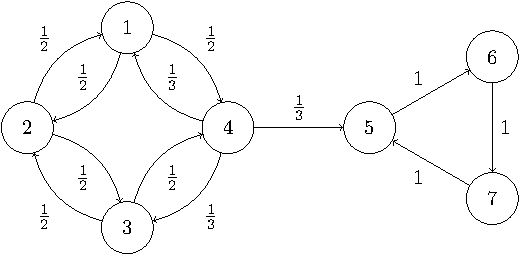
\includegraphics{math2750_files/figure-latex/periods-1} 

}

\caption{Transition for an aperiodic irreducible Markov chain.}\label{fig:periods}
\end{figure}

Importantly, we can't return from the triangle side back to the circle side. We thus see there are two communicating classes: \(\{1,2,3,4\}\), which is open, and \(\{5,6,7\}\), which is closed. The Markov chain is not irreducible, and there are no absorbing states.

The circle side swaps between odd and even states (until exiting from \(4\) to \(5\)), so states \(1\),\(2\), \(3\) and \(4\) all have period \(2\). The triangle side cycles around with certainty, meaning that states \(5\), \(6\), and \(7\) all have period \(3\).

\end{example}

You may have noticed in these examples that, within a communicating class, every state has the same period. In fact, it's always the case that states in the same class have the same period.

\begin{theorem}
\protect\hypertarget{thm:class-period}{}\label{thm:class-period}

All states in a communicating class have the same period.

Formally: Consider a Markov chain on a state space \(\mathcal S\) with transition matrix \(\mathsf P\). If \(i,j\in\mathcal S\) are such that \(i \leftrightarrow j\), then \(d_i = d_j\).

\end{theorem}

In particular, in an irreducible Markov chain, all states have the same period \(d\). We say that an irreducible Markov chain is \textbf{periodic} if \(d>1\) and \textbf{aperiodic} if \(d=1\).

\begin{proof}

Let \(i,j\) be such that \(i \leftrightarrow j\). We want to show that \(d_i = d_j\). First we'll show that \(d_i \leq d_j\), and then we'll show that \(d_j \leq d_i\), and thus conclude that they're equal.

Since \(i\leftrightarrow j\), there exist \(n,m\) such that \(p_{ij}(n)>0\) and \(p_{ji}(m)>0\). Then, by the Chapman--Kolmogorov equations,
\[ p_{ii}(n+m) =  \sum_{k \in \mathcal S} p_{ik}(n) p_{ki}(m) \geq p_{ij}(n) p_{ji}(m) > 0 .  \]
So \(d_i\) divides \(n+m\).

Let \(r\) be such that \(p_{jj}(r)>0\). Then, by the same Chapman-Kolmogorov argument,
\[
    p_{ii}(n+m+r)\geq  p_{ij}(n) p_{jj}(r) p_{ji}(m) > 0,
    \]
because we can get from \(i\) to \(i\) by going \(i \to j \to j \to i\).
Hence \(d_i\) divides \(n+m+r\).

\begin{verbatim}
But if $d_i$ divides both $n+m$ and $n+m+r$, it must be that $d_i$ divides $r$ also. So whenever $p_{jj}(r)>0$, we have that $d_i$ divides $r$. Since $d_i$ is a common divisor of all the $r$s with $p_{jj}(r)>0$, it can't be any bigger that the *greatest* common divisor of all those $r$s. But that greatest common divisor is by definition $d_j$, the period of $j$. So $d_i \leq d_j$.
\end{verbatim}

Repeating the same argument but with \(i\) and \(j\) swapped over, we get \(d_j\leq d_i\) too, and we're done.

\end{proof}

\textbf{In the next section}, we look at two problems to do with ``hitting times'': What is the probability we reach a certain state, and how long on average does it take us to get there?

\hypertarget{S08-hitting-times}{%
\section{Hitting times}\label{S08-hitting-times}}

\begin{itemize}
\tightlist
\item
  Definitions: Hitting probability, expected hitting time, return probability, expected return time
\item
  Finding these by conditioning on the first step
\item
  Return probability and expected return time for the simple random walk
\end{itemize}

\hypertarget{hitting-definitions}{%
\subsection{Hitting probabilities and expected hitting times}\label{hitting-definitions}}

In \protect\hyperlink{S03-gamblers-ruin}{Section 3} and \protect\hyperlink{S04-ldes}{Section 4}, we used conditioning on the first step to find the ruin probability and expected duration for the gambler's ruin problem. Here, we develop those ideas for general Markov chains.

\begin{definition}
\protect\hypertarget{def:hitting-defs}{}\label{def:hitting-defs}

Let \((X_n)\) be a Markov chain on state space \(\mathcal S\). Let \(H_{A}\) be a random variable representing the \textbf{hitting time} to hit the set \(A \subset \mathcal S\), given by
\[ H_{A} = \min \big\{n \in \{0,1,2,\dots\} : X_n \in A  \big\}  . \]
The most common case we'll be interested in will be when \(A = \{j\}\) is just a single state, so
\[ H_{j} = \min \big\{n \in \{0,1,2,\dots\} : X_n = j  \big\}  . \]
(We use the convention that \(H_A = \infty\) if \(X_n \not\in A\) for all \(n\).)

The \textbf{hitting probability} \(h_{iA}\) of the set \(A\) starting from state \(i\) is
\[ h_{iA} = \mathbb P(X_n \in A \text{ for some $n \geq 0$} \mid X_0 = i) = \mathbb P(H_A < \infty \mid X_0 = i) .  \]
Again, the most common case of interest is \(h_{ij}\) the hitting probability of state \(j\) starting from state \(i\).

The \textbf{expected hitting time} \(\eta_{iA}\) of the set \(A\) starting from state \(i\) is
\[ \eta_{iA} = \mathbb E(H_A \mid X_0 = i) .  \]
Clearly \(\eta_{iA}\) can only be finite if \(h_{iA} = 1\).

\end{definition}

The short summary of this is:

\begin{itemize}
\tightlist
\item
  The \textbf{hitting probability} \(h_{ij}\) is the probability we hit state \(j\) starting from state \(i\).
\item
  The \textbf{expected hitting time} \(\eta_{ij}\) is the expected time until we hit state \(j\) starting from state \(i\).
\end{itemize}

The good news us that we already know how to find hitting probabilities and expected hitting times, because we already did it for the \protect\hyperlink{S03-gamblers-ruin}{gambler's ruin problem}! The way we did it then is that we first found equations for hitting probabilities or expected hitting times by conditioning on the first step, and then we solved those equations. We do the same here for other Markov chains.

Let's see an example of how to find a hitting probability.

\begin{example}
\protect\hypertarget{exm:hitting1}{}\label{exm:hitting1}

\emph{Consider a Markov chain with transition matrix}
\[ \begin{pmatrix}
\frac15 & \frac15 & \frac15 & \frac25 \\
0 & 1 & 0 & 0 \\
0 & \frac12 & 0 & \frac12 \\
0 & 0 & 0 & 1
\end{pmatrix} . \]
\emph{Calculate the probability that the chain is absorbed at state \(2\) when started from state \(1\).}

This is asking for the hitting probability \(h_{12}\). We use -- as ever -- a conditioning on the first step argument. Specifically, we have
\begin{align}
  h_{12} &= p_{11} h_{12} + p_{12} h_{22} + p_{13} h_{32} + p_{14} h_{42}  \\
         &= \tfrac 15 h_{12} + \tfrac 15 h_{22} + \tfrac 15 h_{32} + \tfrac 25 h_{42}  \label{eq:hiteq}
\end{align}
This is because, starting from 1, there's a \(p_{11} = \frac15\) probability of staying at 1; then by the Markov property it's like we're starting again from 1, so the hitting probability is still \(h_{12}\). Similarly, there's a \(p_{12} = \frac15\) probability of moving 2; then by the Markov property it's like we're starting again from 2, so the hitting probability is still \(h_{22}\). And so on.

Since \eqref{eq:hiteq} includes not just \(h_{12}\) but also \(h_{22}\), \(h_{32}\) and \(h_{42}\), we need to find equations for those too. Clearly we have \(h_{22} = 1\), as we are ``already there''. Also, \(h_{42} = 0\), since 4 is an absorbing state. For \(h_{32}\), another ``condition on the first step'' argument gives
\[ h_{32} = p_{32}h_{22} + p_{34}h_{42} = \tfrac12 h_{22} + \tfrac12 h_{42} = \tfrac12 ,\]
where we substituted in \(h_{22} = 1\) and \(h_{42} = 0\).

Substituting \(h_{22} = 1\), \(h_{32} = \frac12\) and \(h_{42} = 0\) all into \eqref{eq:hiteq}, we get
\[ h_{12} = \tfrac15 h_{12} + \tfrac15 + \tfrac15 \tfrac12 = \tfrac15 h_{12} + \tfrac{3}{10}. \]
Hence \(\frac45 h_{12} = \frac{3}{10}\), so the answer we were after is \(h_{12} = \frac38\).

\end{example}

So the technique to find hitting probability \(h_{ij}\) from \(i\) to \(j\) is:

\begin{enumerate}
\def\labelenumi{\arabic{enumi}.}
\tightlist
\item
  Set up equations for all the hitting probabilities \(h_{kj}\) to \(j\) by conditioning on the first step.
\item
  Solve the resulting simultaneous equations.
\end{enumerate}

It is recommended to derive equations for hitting probabilities from first principles by conditioning on the first step, as we did in the example above. However, we can state what the general formula is: by the same conditioning method, we get
\[ h_{iA} = \begin{cases} \displaystyle\sum_{j \in \mathcal S} p_{ij} h_{jA} & \text{if $i \not\in A$} \\
1 & \text{if $i \in A$.} \end{cases} \]
It can be shown that, if these equations have multiple solutions, then the hitting probabilities are in fact the smallest non-negative solutions.

Now an example for expected hitting times.

\begin{example}
\protect\hypertarget{exm:hitting2}{}\label{exm:hitting2}

\emph{Consider \protect\hyperlink{S06-example1}{the simple no-claims discount chain from Lecture 6}, which had transition matrix}
\[ \mathsf P =\begin{pmatrix}
    \tfrac14 &\tfrac34 & 0\\
    \tfrac14 &0 & \tfrac34\\
    0 &\tfrac14 & \tfrac34\\
    \end{pmatrix} .\]
\emph{Given we start in state 1 (no discount), find the expected amount of time until we reach state 3 (50\% discount).}

This question asks us to find \(\eta_{13}\). We follow the general method, and start by writing down equations for all the \(\eta_{i3}\)s.

Clearly we have \(\eta_{33} = 0\).
For the others, we condition on the first step to get
\begin{align*}
\eta_{13} = 1 + \tfrac14 \eta_{13} + \tfrac34 \eta_{23} \qquad &\Rightarrow \qquad \phantom{-}\tfrac34 \eta_{13} - \tfrac34\eta_{23} = 1 ,\\
\eta_{23} = 1 + \tfrac14 \eta_{13} + \tfrac34 \eta_{33} \qquad &\Rightarrow \qquad  - \tfrac14\eta_{13} + \phantom{\tfrac34}\eta_{23} = 1 .
\end{align*}
This is because the first step takes time \(1\), then we condition on what happens next -- just like we did for the gambler's ruin.

The first equation plus three-quarters times the second gives
\[ \big(\tfrac34 - \tfrac34\tfrac14\big) \eta_{13} = \tfrac{9}{16}\eta_{13} = 1 + \tfrac34 = \tfrac 74 = \tfrac{28}{16} ,\]
which has solution \(\eta_{13} = \tfrac{28}{9} = 3.11\).

\end{example}

Similarly, if we need to, we can give a general formula
\[ \eta_{iA} = \begin{cases} 1 + \displaystyle\sum_{j \in \mathcal S} p_{ij} \eta_{jA} & \text{if $i \not\in A$} \\
0 & \text{if $i \in A$.} \end{cases} \]
Again, if we have multiple solutions, the expected hitting times are the smallest non-negative solutions.

\hypertarget{return-times}{%
\subsection{Return times}\label{return-times}}

Under the definitions above, the hitting probability and expected hitting time to a state from itself are always \(h_{ii} = 1\) and \(\eta_{ii} = 0\), as we're ``already there''.

In this case, it can be interesting to look instead at the random variable representing the \textbf{return time},
\[ M_i = \min \big\{n \in \{1,2,\dots\} : X_n = i  \big\} . \]
Note that this only considers times \(n = 1, 2, \dots\) not including \(n = 0\), so is the \emph{next} time we come back, after \(n = 0\).

We then have the \textbf{return probability} and \textbf{expected return time}
\begin{gather*} m_{i} = \mathbb P(X_n = i  \text{ for some $n \geq 1$} \mid X_0 = i) = \mathbb P(M_i < \infty \mid X_0 = i) ,  \\
 \mu_{i} = \mathbb E(M_i \mid X_0 = i) .  \end{gather*}

Just as before, we can find these by conditioning on the first step. The general equations are
\[
      m_i = \sum_{j \in \mathcal S} p_{ij}h_{ji} , \qquad
      \mu_i = 1 + \sum_{j \in \mathcal S} p_{ij}\eta_{ji},
  \]
where, if necessary, we take the minimal non-negative solution again.

\hypertarget{return-rw}{%
\subsection{Hitting and return times for the simple random walk}\label{return-rw}}

We now turn to hitting and return times for the simple random walk, which goes up with probability \(p\) and down with probability \(q = 1-p\). This material is mandatory and is examinable, but is a bit technical; students who are struggling or have fallen behind might make a tactical decision just to read the two summary theorems below and come back to the details at a later date.

Let's start with hitting probabilities. Without loss of generality, we look at \(h_{i0}\), the probability the random walk hits 0 starting from \(i\).
We will assume that \(i > 0\). For \(i < 0\), we can get the desired result by looking at the random walk ``in the mirror'' -- that is, by swapping the role of \(p\) and \(q\), and treating the positive value \(-i\).

For an initial condition, it's clear we have \(h_{00} = 1\).

For general \(i > 0\), we condition on the first step, to get
\[ h_{i0} = ph_{i+1\, 0} + qh_{i-1\, 0} .  \]
We recognise this equation from the gambler's ruin problem, and recall that we have to treat the cases \(p \neq \frac12\) and \(p = \frac12\) separately.

When \(p \neq \frac12\), the general solution is \(h_{i0} = A + B\rho^i\), where \(\rho = q/p \neq 1\), as before. The initial condition \(h_{00} = 1\) gives \(A = 1-B\), so we have a family of solutions
\[ h_{i0} = (1 - B) + B\rho^i = 1 + B(\rho^i - 1) . \]

In the gambler's ruin problem we had another boundary condition to find \(B\). Here we have no other conditions, but we can use the minimality condition that the hitting probabilities are the smallest non-negative solution to the equation. This minimal non-negative solution will depend on whether \(\rho > 1\) or \(\rho < 1\).

When \(\rho > 1\), so \(p < \frac12\), the term \(\rho^i\) tends to infinity. Thus the minimal non-negative solution will have to take \(B = 0\), because taking \(B < 0\) would eventually give a negative solution, while \(B = 0\) gives the smallest of the non-negative solutions. Hence the solution is \(h_{i0} = 1 + 0(\rho^i-1) = 0\), meaning we hit 0 with certainty. This makes sense, because for \(p < \frac12\) the random walk ``drifts'' to the left, and eventually gets back to 0.

When \(\rho < 1\), so \(p > \frac12\), we have that \(\rho^i - 1\) is negative and tends to \(-1\). So to get a small solution we want \(B\) large and positive, but keeping the solution non-negative limits us to \(B \leq 1\), so the minimality condition is achieved at \(B = 1\). The solution is \(h_{i0} = 1 + 1(\rho^i - 1) = \rho^i\). This is strictly less than 1 as expected, because for \(p > 1/2\), the random walk drifts to the right, so might drift further and further away from 0 and not come back.

For \(p = \frac12\), so \(\rho = 1\), we recall the general solution \(h_{i0} = A + Bi\). The condition \(h_{00} = 1\) gives \(A = 1\), so \(h_{i0} = 1 + Bi\). Because \(i\) is positive, to get the answer to be small we want \(B\) to be small, but non-negativity limits us to \(B\) positive, so the minimal non-negative solution takes \(B = 0\). This gives \(h_{i0} = 1 + 0i = 0\), so we will always get back to 0.

In conclusion, we have the following. (Recall that we get the result for \(i < 0\) by swapping the role of \(p\) and \(q\), and treating the positive value \(-i\).)

\begin{theorem}
\protect\hypertarget{thm:rw-hitting}{}\label{thm:rw-hitting}

Consider a random walk with up probability \(p \neq 0, 1\). Then the hitting probabilities to 0 are givin by, for \(i > 0\),
\[ h_{i0} = \begin{cases} \left(\displaystyle\frac{q}{p}\right)^i & \text{if $p > \frac12$} \\ \ 1 & \text{if $p \leq \frac12$,} \end{cases} \]
and for \(i < 0\) by
\[ h_{i0} = \begin{cases} \left(\displaystyle\frac{p}{q}\right)^{-i} & \text{if $p < \frac12$} \\ \ 1 & \text{if $p \geq \frac12$.} \end{cases} \]

\end{theorem}

Now we look at return times. What is the return probability to 0 (or, by symmetry, to any state \(i \in \mathbb Z\))? By conditioning on the first step, \(m_0 = ph_{1\,0} + qh_{-1\,0}\), and we've calculated those hitting times above. We have
\[ m_0 = \begin{cases} p\times 1 \hspace{0.4em}+ q\times 1 \hspace{0.4em}= 1 & \text{if $p = \frac12$} \\
p \times \displaystyle\frac qp + q\times 1 \hspace{0.4em}= 2q < 1 & \text{if $p > \frac12$} \\
p\times 1 \hspace{0.4em} + q \times \displaystyle\frac pq = 2p < 1 & \text{if $p < \frac12$.}\end{cases} \]

So for the simple symmetric random walk (\(p = \frac12\)) we have \(m_i = 1\) and are certain to return to the initial state again and again, while for \(p \neq \frac12\), we have \(m_i < 1\) and we might never return.

What about the expected return times \(\mu_{0}\)? For \(p \neq \frac12\), we have \(\mu_{0} = \infty\), since \(m_0 < 1\) and we might never come back. For \(p = \frac12\), though, \(m_0 = 1\), so we have work to do.

To get the expected return time for \(p = \frac12\), we'll need the expected hitting times for for \(p = \frac12\) too. Conditioning on the first step gives the equation
\[ \eta_{i0} = 1 + \tfrac12\eta_{i+1\,0} + \tfrac12\eta_{i-1\,0} , \]
with initial condition \(\eta_{00} = 0\). We again recognise from the gambler's ruin problem the general solution \(\eta_{i0} = A + Bi -i^2\). The initial condition gives \(A = 0\), so \(\eta_{i0} = Bi - i^2 = i(B-i)\). Then non-negativity demands \(B = \infty\), as any other value would get drowned out by the large negative value \(-i^2\), making the whole expression negative for big enough \(i\). Thus we have \(\eta_{i0} = \infty\).

Then we see easily that the return time is
\[ \mu_0 = 1 + \tfrac12 \eta_{1\,0} + \tfrac12 \eta_{-1\,0} = 1 + \tfrac12 \infty + \tfrac12 \infty = \infty. \]
So for \(p = \frac12\), while the random walk always return, it may take a very long time to do so.

In conclusion, this is what we found out:

\begin{theorem}
\protect\hypertarget{thm:rw-summary}{}\label{thm:rw-summary}

Consider the simple random walk with \(p \neq 0,1\). Then for all states \(i\) we have the following:

\begin{itemize}
\tightlist
\item
  For \(p \neq \frac12\), the return probability \(m_i\) is strictly less than 1, so the expected return time \(\mu_i\) is infinite.
\item
  For the simple symmetric random walk with \(p = \frac12\), the return probability \(m_i\) is equal to 1, but the expected return time \(\mu_i\) is still infinite.
\end{itemize}

\end{theorem}

\textbf{In the next section}, we look at how the return probabilities and expected return times characterise which states continue to be visited by a Markov chain in the long run.

\hypertarget{P04}{%
\section*{Problem sheet 4}\label{P04}}
\addcontentsline{toc}{section}{Problem sheet 4}

\commfalse

You should attempt all these questions and write up your solutions in advance of your workshop in week 5 (Monday 22 or Tuesday 23 February) where the answers will be discussed.

\textbf{1.} Consider the Markov chain with state space \(\mathcal S = \{1,2,3,4\}\) and transition matrix
\[ \mathsf P = \begin{pmatrix} 1 & 0 & 0 & 0 \\
1-\alpha & 0 & \alpha & 0 \\
0 & \beta & 0 & 1-\beta \\
0 & 0 & 0 & 1 \end{pmatrix}   \]
where \(0 < \alpha, \beta < 1\).

\textbf{(a)} Draw a transition diagram for this Markov chain.

\begin{myanswers}

\emph{Solution.}

\begin{figure}

{\centering 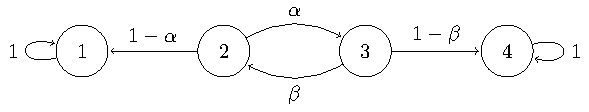
\includegraphics{math2750_files/figure-latex/Q41-1} 

}

\caption{Transition diagram for Question 1.}\label{fig:Q41}
\end{figure}

\end{myanswers}

\textbf{(b)} What are the communicating classes for this Markov chain? Is the chain irreducible. Which classes are closed? Which states are absorbing?

\begin{myanswers}

\emph{Solution.} Clearly \(\{1\}\) and \(\{4\}\) are closed communicating classes, so \(1\) and \(4\) are absorbing states. The other class, \(\{2,3\}\) is not closed. Because there are multiple classes, the chain is not irreducible.

\end{myanswers}

\textbf{(c)} Find the hitting probability \(h_{21}\) that, starting from state \(2\), the chain hits state \(1\).

\begin{myanswers}

\emph{Solution.} It's clear that \(h_{11} = 1\) and \(h_{41} = 0\). Then, by condtioning on the first step, we have
\begin{gather*}
    h_{21} = \alpha h_{31} + (1-\alpha) h_{11} = \alpha h_{31} + 1 - \alpha \\
    h_{31} = \beta h_{21} + (1-\beta) h_{41} = \beta h_{21} .
    \end{gather*}
Substituting the second equation into the first, we get \(h_{21} = \alpha\beta h_{21} + 1 - \alpha\), so
\[ h_{21} = \frac{1-\alpha}{1-\alpha\beta}  . \]

\end{myanswers}

\textbf{(d)} What is the expected time, starting from state \(2\), to reach an absorbing state?

\begin{myanswers}

\emph{Solution.} Let's write \(A = \{1,4\}\) for the absorbing states, and \(\eta_{iA}\) for the time to reach an absorbing state starting from state \(i\). Clearly \(\eta_{1A} = \eta_{4A} = 0\). By conditioning on the first step, we have
\begin{gather*}
    \eta_{2A} = 1 + \alpha \eta_{3A} + (1-\alpha) \eta_{1A} = 1 + \alpha \eta_{3A}  \\
    \eta_{3A} = 1 + \beta \eta_{2A} + (1-\beta) \eta_{4A} = 1+\beta \eta_{2A} .
    \end{gather*}
Substituting the second equation into the first gives
\(\eta_{2A}= 1 + \alpha + \alpha\beta \eta_{2A}\), so
\[ \eta_{2A} = \frac{1+\alpha}{1-\alpha\beta}  . \]

\end{myanswers}

\textbf{2.}
Consider the Markov chain with state space \(\mathcal S = \{1,2,3,4,5\}\) and transition matrix
\[ \mathsf P = \begin{pmatrix} 0 & \frac13 & \frac23 & 0 & 0 \\
                0 & 0 & 0 & \frac14 & \frac34 \\
                0 & 0 & 0 & \frac14 & \frac34 \\
                1 & 0 & 0 & 0 & 0 \\
                1 & 0 & 0 & 0 & 0 \end{pmatrix} . \]

\textbf{(a)} Draw a transition diagram for this Markov chain.

\begin{myanswers}

\emph{Solution.}

\begin{figure}

{\centering 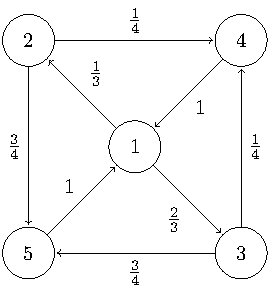
\includegraphics{math2750_files/figure-latex/Q42-1} 

}

\caption{Transition diagram for Question 2.}\label{fig:Q42}
\end{figure}

\end{myanswers}

\textbf{(b)} Show that the chain is irreducible.

\begin{myanswers}

\emph{Solution.} We have paths \(1 \to 2 \to 4 \to 1\) and \(1 \to 3 \to 5 \to 1\), so every state communicates with state 1, so by transitivity every state communicates with every other state.

\end{myanswers}

\textbf{(c)} What are the periods of the states?

\begin{myanswers}

\emph{Solution.} Any path from \(1\) to \(1\) goes \(1 \to \{2 \text{ or }3\} \to \{4 \text{ or }5\} \to 1\). So \(p_{11}^{(n)} > 0\) if and only if \(n\) is a multiple of \(3\). So state \(1\) has period \(d_1 = 3\). Because the chain is irreducible, all other states have period \(3\) too.

\end{myanswers}

\textbf{(d)} Find the expected hitting times \(\eta_{i1}\) from each state \(i\) to \(1\), and the expected return time \(\mu_i\) to \(1\).

\begin{myanswers}

\emph{Solution.} We could do this through a traditional conditioning on the first step argument. But in fact, the cyclic structure \(1 \to \{2 \text{ or }3\} \to \{4 \text{ or }5\} \to 1\) makes it immediately clear that \(\eta_11 = 0\), \(\eta_{41}=\eta_{51} = 1\), \(\eta_{21} = \eta_{31} = 2\), and \(\mu_1 = 3\).

\end{myanswers}

::::: \{.myq\}
\textbf{3.}

Show that every Markov chain on a finite state space \(\mathcal S\) has at least one closed communicating class.

\begin{myanswers}

\emph{Solution.} For communicating classes \(C,D\), let's write \(C \to D\) if there is an \(i \in C\) and \(j \in D\) with \(i \to j\). Note that we can't have both \(C \to D\) and \(D \to C\) is \(C\) and \(D\) are distinct classes. This is because there would be \(i_1, j_2 \in C\) and \(i_2, j_1 \in D\) such that \(i_1 \to i_2 \to j_1 \to j_2 \to i_1\), so they would be the same class. Let's also note that there are a finite number of classes \(m\).

Pick a class \(C_1\). If \(C_1\) is closed, we are done; otherwise \(C_1 \to C_2\) for some other class \(C_2\). If \(C_2\) is closed, we are done; otherwise \(C_2 \to C_3\) for some class \(C_3\) different to \(C_1\) and \(C_2\). (It can't be \(C_1\) by the arguemnt.) We repeat: if \(C_k\) is closed, we are done; otherwise there's a new class \(C_{k+1}\) with \(C_k \to C_{k+1}\). Repeating, we eventually find a closed class: we either terminate before step \(m\) at a closed class, or otherwise \(C_m\) must be closed, as none of the previous \(m-1\) classes can be accessible from it, by our earlier example.

\end{myanswers}

\textbf{(b)} Give an example of a Markov chain that has no closed communicating classes.

\begin{myanswers}

\emph{Solution.} By part (a), the state space must be infinite. Here's one example: take \(\mathcal S = \mathbb Z\), and \(X_{n+1} = X_n + 1\) with probability \(1\). There are no states \(i\) and \(j\) such that \(i \leftrightarrow j\) except for states communicating with themselves, so each state is a separate class. But clearly there is no absorbing state.

\end{myanswers}

\textbf{4.} Prove or give a counterexample: The period of a state \(i\) is the smallest \(d > 0\) such that \(p_{ii}(d) > 0\).

\textbf{5.} Consider the simple random walk with \(p < \frac12\), and let \(i > 0\). Show that
\(\eta_{i0} = i/(q-p)\).

\textbf{6.} Consider the Markov chain with the following transition matrix and transition diagram:

\begin{figure}

{\centering 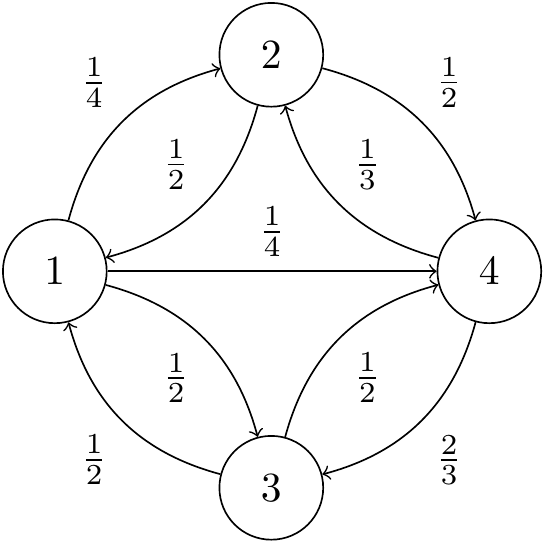
\includegraphics{math2750_files/figure-latex/Q45-1} 

}

\caption{Transition diagram for Question 5.}\label{fig:Q45}
\end{figure}

\[ \mathsf P = \begin{pmatrix} 0 & \frac14 & \frac12 & \frac14 \\
               \frac12 & 0& 0& \frac12 \\
               \frac12 & 0& 0& \frac12 \\
               0 & \frac13 & \frac23 & 0 \end{pmatrix} \]

The Markov chain starts from state \(1\).

\textbf{(a)} What is the probability that we hit state \(2\) before we hit state \(3\)?

\begin{myanswers}

\emph{Solution.} Write \(k_i\) for the probability we hit state \(2\) before state \(3\) starting from \(i\). Then clearly \(k_2 = 1\) (since we've hit \(2\) first) and \(k_3 = 0\) (since we've hit \(3\) first). Further, by conditioning on the first step, \(k_4 = \frac13 k_2 + \frac23 k_3 = \frac13\), and
\[ k_1 = \tfrac14 k_2 + \tfrac12k_3 + \tfrac14 k_4   = \tfrac14 + \tfrac14 k_4 = \tfrac14 + \tfrac14\tfrac13 = \tfrac13 . \]
The desired solution is \(k_1 = \frac13\).

\end{myanswers}

\textbf{(b)} What is the expected time until we hit the first of set \(\{2,3\}\)?

\begin{myanswers}

Let \(A = \{2,3\}\), and \(\eta_{iA}\) be the expected time until hitting the first of states \(2\) and \(3\) starting from \(i\). Clearly \(\eta_{2A} = \eta_{3A} = 0\). By conditioning on the first step, \(\eta_{4A} = 1+ \frac13 \eta_{2A} + \frac23 \eta_{3A} = 1\), and
\[ \eta_{1A} = 1 + \tfrac14 \eta_{2A} + \tfrac12\eta_{3A} + \tfrac14 \eta_{4A} = 1 + \tfrac14 = \tfrac54 .        \]
The desired solution is \(\eta_{1A} = \tfrac54\).

\end{myanswers}

\hypertarget{computing}{%
\section*{Computational worksheets}\label{computing}}
\addcontentsline{toc}{section}{Computational worksheets}

\begin{itemize}
\tightlist
\item
  \textbf{Computational Worksheet 1:} \href{computing/C1.html}{{[}HTML format{]}} \href{computing/C1.Rmd}{{[}Rmd format{]}}
\end{itemize}

\hypertarget{C-about}{%
\subsection*{About the computational worksheets}\label{C-about}}
\addcontentsline{toc}{subsection}{About the computational worksheets}

These computational worksheets are an opportunity to learn more about Markov chains through simulation using R.

This first worksheet is not an assessed part of the course, but it is for you to learn and practice. The second worksheet \emph{is} an assessed part of the course, and counts for 3\% of your grade on this course. A report on Worksheet 2 will be due on \textbf{Thursday 18 March} (week 8) at 2pm. The material in these worksheets is examinable.

I recommend working on Computational Worksheet 1 in weeks 3 or 4, and on Computational Worksheet 2 in weeks 6 or 7. I estimate that each worksheet may take about 2 hours to work through.

You will have two computational drop-in sessions available with Muyang Zhang. These drop-in sessions are optional opportunities for you to come along to ask for help if you are stuck or want to know more. These sessions will happen on Teams. The sessions may appear in your timetable as ``Practicals''. It is important that you work through most of the worksheet \emph{before} your drop-in session, as this will be your main opportunity to ask for help. (You can also use the module discussion board on Teams.) The dates of the drop-in sessions are:

\begin{itemize}
\tightlist
\item
  Computational Worksheet 1: Monday 15 -- Wednesday 17 February (week 4)
\item
  Computational Worksheet 2: Monday 8 -- Wednesday 10 March (week 7)
\end{itemize}

Note that the Worksheet 2 practical sessions are the week before the deadline, so it's in your benefit to start working on that worksheet early.

The computational worksheets are available in two formats:

\begin{itemize}
\tightlist
\item
  First, as an easy-to-read \textbf{HTML file}. You should open this in a web browser.
\item
  Second, as a file with the suffix \textbf{.Rmd}. This can be read as a plain text file. However, I recommend downloading this file and opening it in RStudio. This will make it easy to run the R code included in the file, by clicking the green ``play'' button by each chunk of R code. (These files is written in a language called ``\href{https://www.stat.cmu.edu/~cshalizi/rmarkdown/}{R Markdown}'', which you could choose to use for writing your report.)
\end{itemize}

\hypertarget{R-access}{%
\subsection*{How to access R}\label{R-access}}
\addcontentsline{toc}{subsection}{How to access R}

These worksheets use the statistical programming language \textbf{R}. Use of R is mandatory. I recommend interacting with R via the program \textbf{RStudio}, although this is optional. There are various ways to access R and RStudio.

\begin{itemize}
\tightlist
\item
  You may already have R and RStudio installed on your own computer.
\item
  You can install R and RStudio on your own computer now if you haven't previously. You should first \href{https://cran.rstudio.com/}{download R from the Comprehensive R Archive Network}, and then \href{https://rstudio.com/products/rstudio/download/\#download}{download ``RStudio Desktop'' from rstudio.com}. Remember to download and install R first, and only then to download and install RStudio.
\item
  The \href{https://rstudio.cloud/}{RStudio Cloud} is like ``Google Docs for R''. You can get 15 hours a month for free, which should be more than enough for these worksheets. Because this doesn't require installation, it's good for Chromebooks or computers where you don't have full installation rights.
\item
  If you are in Leeds, all the university computers have R and RStudio installed. However, at the time of writing (5 February 2021), all IT clusters on campus are closed. You can see \href{https://leeds.service-now.com/it?id=clusters}{the latest news on cluster availability here}.
\item
  You can access R and RStudio via the university's \href{https://it.leeds.ac.uk/it?id=kb_article\&sysparm_article=KB0014548}{virtual Windows desktop} or (for those who have a Windows computer) via the university's \href{https://it.leeds.ac.uk/it?id=kb_article\&sysparm_article=KB0014827}{AppsAnywhere} system.
\end{itemize}

\hypertarget{R-background}{%
\subsection*{R background}\label{R-background}}
\addcontentsline{toc}{subsection}{R background}

These worksheets are mostly self-explanatory. However, they do assume a little background. For example, I assume you know how to operate R (for example by opening RStudio and typing commands in the ``console''), and that you know that \texttt{x\ \textless{}-\ c(1,\ 2,\ 3)} creates a vector called \texttt{x} and that \texttt{mean(x)} calculates the mean of the entries of \texttt{x}.

Most students on this course will know R from MATH1710 and MATH1712 or other courses. If you are new to R, I recommend Dr Jochen Voss's ``A Short Introduction to R'' or Dr Arief Gusnanto's ``Introduction to R'', both available from \href{http://www1.maths.leeds.ac.uk/~arief/MATH1712/index.html}{Dr Gusnanto's MATH1712 homepage}.

\end{document}
